\chapter{Antiferromagnetic Ising Model  in Hanoi Networks}
\label{chap-afm}
This chapter uses both computational and theoretical methods to study the dynamics and phase diagrams in antiferromagnetic Ising Model in Hanoi Networks.  First, the motivation of this study is reviewed in \ref{sec:amf-glass-intro}. Then two Monte Carlo methods are used to learn both the equlibrium and non-equlibrium properties for finite system sizes, which is described in \ref{sec:afm-mc}. In Sec. \ref{sec:afm-rg}, renormalization group is set up for both fixed point analysis and equlibrium properties explorations.  Using Monte Carlo methods and RG, spin glass phases, chaos, and a phase diagram are discovered in the model and networks, which is shown in Sec. \ref{sec:afm-results}.  

\section{Spin Glass Phase and Chaos in Antiferromagnets}
\label{sec:amf-glass-intro}
As introduced in Sec. \ref{sec:intro-afm}, the Ising antiferromagnet (AF) is a convenient model of glassy dynamics. With non-random interactions, it can still introduce geometric frustrations through complex structures and may give rise to a spin glass phase and glassy relaxation at low temperatures \cite{villain1977spin, herrero2008afm}. The motivations to this model in hierarchical networks are
\begin{itemize}
\item the antiferromagnetic Ising model (AFM) has been shown to have interesting dynamics \cite{shokef2011}, magnetization plateaus \cite{ohanyan2003mag} , and phase transitions\cite{herrero2008afm}, and even more interesting results are expected from our hierarchical networks;
\item the Hanoi networks are renormalizable and can be studied exactly \cite{boettcher2015classification, Boettcher2011HNNP}, which could provide more insights about the equilibrium dynamics underlying the extremely slow glassy dynamics;
\item the ferromagnetic Ising model in hierarchical networks has been studied  and shows phase transitions in Hanoi networks \cite{brunson2014rg}.
\end{itemize}

It is interesting to see how AFM behaves in these 4 hierarchical networks, HN3, HN5, HNNP, and HN6, whose short-range and long-range bonds create entangled loops of different sizes. These entangled loops can generate complex frustrations and introduce glassy dynamics and even phase transitions. 

First of all,  Wang-Landau algorithm is employed to investigate the energy landscape and the corresponding equilibrium behaviors for a range of different system sizes. Then simulated annealing is used to explore the dynamical behaviors, and an extremely slow relaxation is discovered at low temperatures, which also has a power-law scaling to different annealing schedules.  In addition to these two Monte Carlo methods, renormalization group is the main focus to study the equilibrium properties in the thermodynamic limit and to compare with the results from simulated annealing and Wang-Landau sampling. We discover three phases (ferromagnetic, paramagnetic, and spin glass phases) and an interesting phase diagram of the transitions. 


\section{Monte Carlo Methods}
\label{sec:afm-mc}
Similarly to the methods in Chater \ref{chap-jamming}, two Monte Carlo methods are used. Wang-Landau sampling is used to estimate the density of states, its energy landscape, and further equlibrium properties for finite system sizes; while simulated annealing can simulate experiments and the glassy dynamics.
 
\subsection{Wang-Landau Sampling}
Wang-Landau sampling is first introduced to estimate the density of states in ferromagnetic Ising model \cite{Wang2001}. Here we use it to calculate the density of states $g_{n}$ of AFM in
these 4 networks. Comparing to tradiation Ising model, AFM in Hanoi networks has entangled geometric frustractions, so we expect slower convergence and more computational complexity. From the experience in Jamming systems sampling, the sampling procedure for AFM in Hanoi networks is: 
\begin{enumerate}
\item Initially, set all unknown density of states $\{g_{E}=1\}$ and the
histogram $\{H_{E}=0\}$ for all energy states $E$, initiate the modification
factor $f=e^1$; 
\item Randomly pick a spin $i$ and flip it with a probability of $\min\left[1,\frac{g_{E_1}}{g_{E_2}}\right]$ where $E_1$ is the current state, and $E_2$ is the state if the spin is flipped;
\item Randomly pick 2 spins and exchange them to explore more states quickly; 
\item Update the $H_{E}$ and $g_{E}$ of the current state, i.e., set $\{H_{E}=H_{E}+1\}$
and $\{g_{E}=g_{E}\times f\}$; 
\item Repeat steps 2 to 4 until the sampling reaches a nearly flat histogram
for the $H_{E}$, then update the modification factor $f=\sqrt{f}$
and reset $\{H_{E}=0\}$; 
\item Stop if $f\le1+10^{-8}$. 
\end{enumerate}

The goal of Step 3 is to facilitate the random walk to explore phase space more broadly and to expedite convergence. We test the computations both with and without Step 3. However, no significant difference of computational efficiency is found, which is very different from the effect in Chapter \ref{chap-jamming}. The difference effect may be due to the intrinsically different interaction models. Exchanging in Jamming system only changes the configuration within the same occupation number $n$; while exchanging in AFM changes both the configuration and the energy, which is equivalent to randomly flipping of 2 sites.  

Due to geometric frustrations, Wang-Landau sampling can only find convergence for system size of up to $N\sim10^{3}$ within $\sim70$ hours of sequential computation. From the density of states, we can calculate the equilibrium thermodynamical properties for the corresponding system sizes, which is included in Sec. \ref{sec:afm-results}. 

\subsection{Simulated Annealing}
One of the most interesting phenomena in AFM is its glassy dynamics which can be learnt using Monte Carlo simulation. In this work, a canonical Monte Carlo method, Simulated Annealing ~\cite{SA}, is used to explore the dynamics from high to low temperatures. 

Similarly to the study of jamming in Chapter ~\ref{chap-jamming}, the Monte Carlo simulation can be considered as an experiment. The corresponding experiment is randomly flipping spins in the networks under a certain temperature $T$.  The standard procedure of the simulated annealing ~\cite{Vcerny1985} is adopted in this model. In the simulation, the procedure of the annealing algorithm is: 
\begin{enumerate}
\item Initially, start with a high temperature $T_{0}=10$ ; 
\item Randomly pick a spin on a lattice site $n$ to propose a flip; 
\item Flip the selected spin with a probability of $\min\left[1, \exp(-\Delta E /T)\right]$ 
where $\Delta E$ is the potential energy change if the spin is flipped; 
\item If exchange is allowed, randomly pick 2 neighbor-spins and exchange with a probability of $\min\left[1, \exp(-\Delta E /T)\right]$; 
\item Increase $T$ by $dT$ every 1 Monte Carlo sweep ($N$ random
updates), where $dT/dt$ (in time-units of $dt=1$ ) is the annealing
schedule and $dT\ll1$; 
\item Repeat steps 2 to 4 until $dT$ reaches a certain low temperature $T=1e-3$. 
\end{enumerate}

Step 4 is not a standard procedure in simulated annealing. The goal is to test the effect of local dynamics, similar to what is used in Chapter \ref{chap-jamming}. However, there is no significant difference in the results, while jamming states are eliminated in Chapter \ref{chap-jamming}. The reason of that may be similar to what we observe in Wang-Landau sampling, which is due to model differences.Detailed results are shown in Sec. \ref{sec:afm-results}.



\section{Renormalization Group}
\label{sec:afm-rg}
Renormalization Group (RG) is applied to these 4 Hanoi networks (HN3, HN5, HNNP, and HN6) which are suitable for decimation transformation in RG. The standard procedure developed for FM model by Boettcher, {\it et. al.} \cite{Boettcher2011HNNP, boettcher2015classification} is used in the AFM here, too. First, the general approach of RG on Hanoi networks is introduced; then the AFM Hamiltonians without and with external fields for these 4 networks is specifically set up and derived for RG.


\subsection{RG on Hanoi Networks}
\label{sec:afm-rghns}
The Hanoi networks are constructed hierarchically which is inherently suitable for RG. As in the stardard RG procedures, the spins in HNs are also hierarchically traced out level by level \cite{Boettcher2011HNNP, brunson2014rg}. For example, the site $n$ in HNs can be described by Eq. \ref{eq:numbering} ( $n(i,j)=2^{i-1}(2j+1)$ ), then the spins are traced out from level $i=1$ level by level. In the end, there is only 3 \enquote{spins} left, and all the Hamiltonian is renormalized to the bonds among these 3  \enquote{spins}.

\begin{figure}
\centering 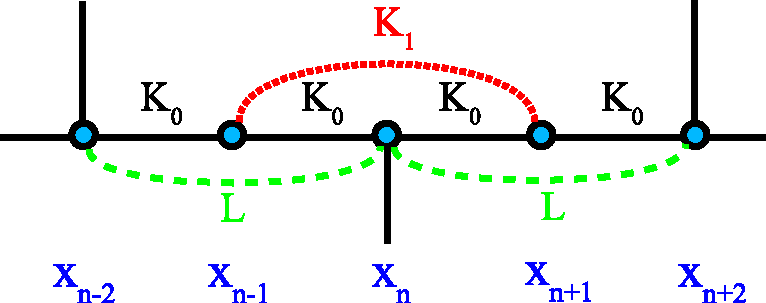
\includegraphics[scale=0.68]{Chapter-3/RG3hanoi}
\protect\caption{HN3 five-spin RG unit with all the couplings among the spins. $K_0$ and $K_1$ are actual bonds (connections) in HN3; while $L$ is emerged in the RG steps.}
\label{fig:afm-hn3rgbefore} 
\end{figure}

In terms of the 4 specific Hanoi network, we start with the most simple one HN3. As shown in Fig. \ref{fig:afm-hn3rgbefore} \cite{Boettcher2011HNNP}, all the couplings are included in a RG unit of 5 spins. The interaction constant on the backbone is $K_0$ ($=\beta J_0$); the coupling through the long-range bonds is $K_1$ ($=\beta J_1$); and $L$ is the emerging interaction which is initially 0.

\begin{figure}
\centering 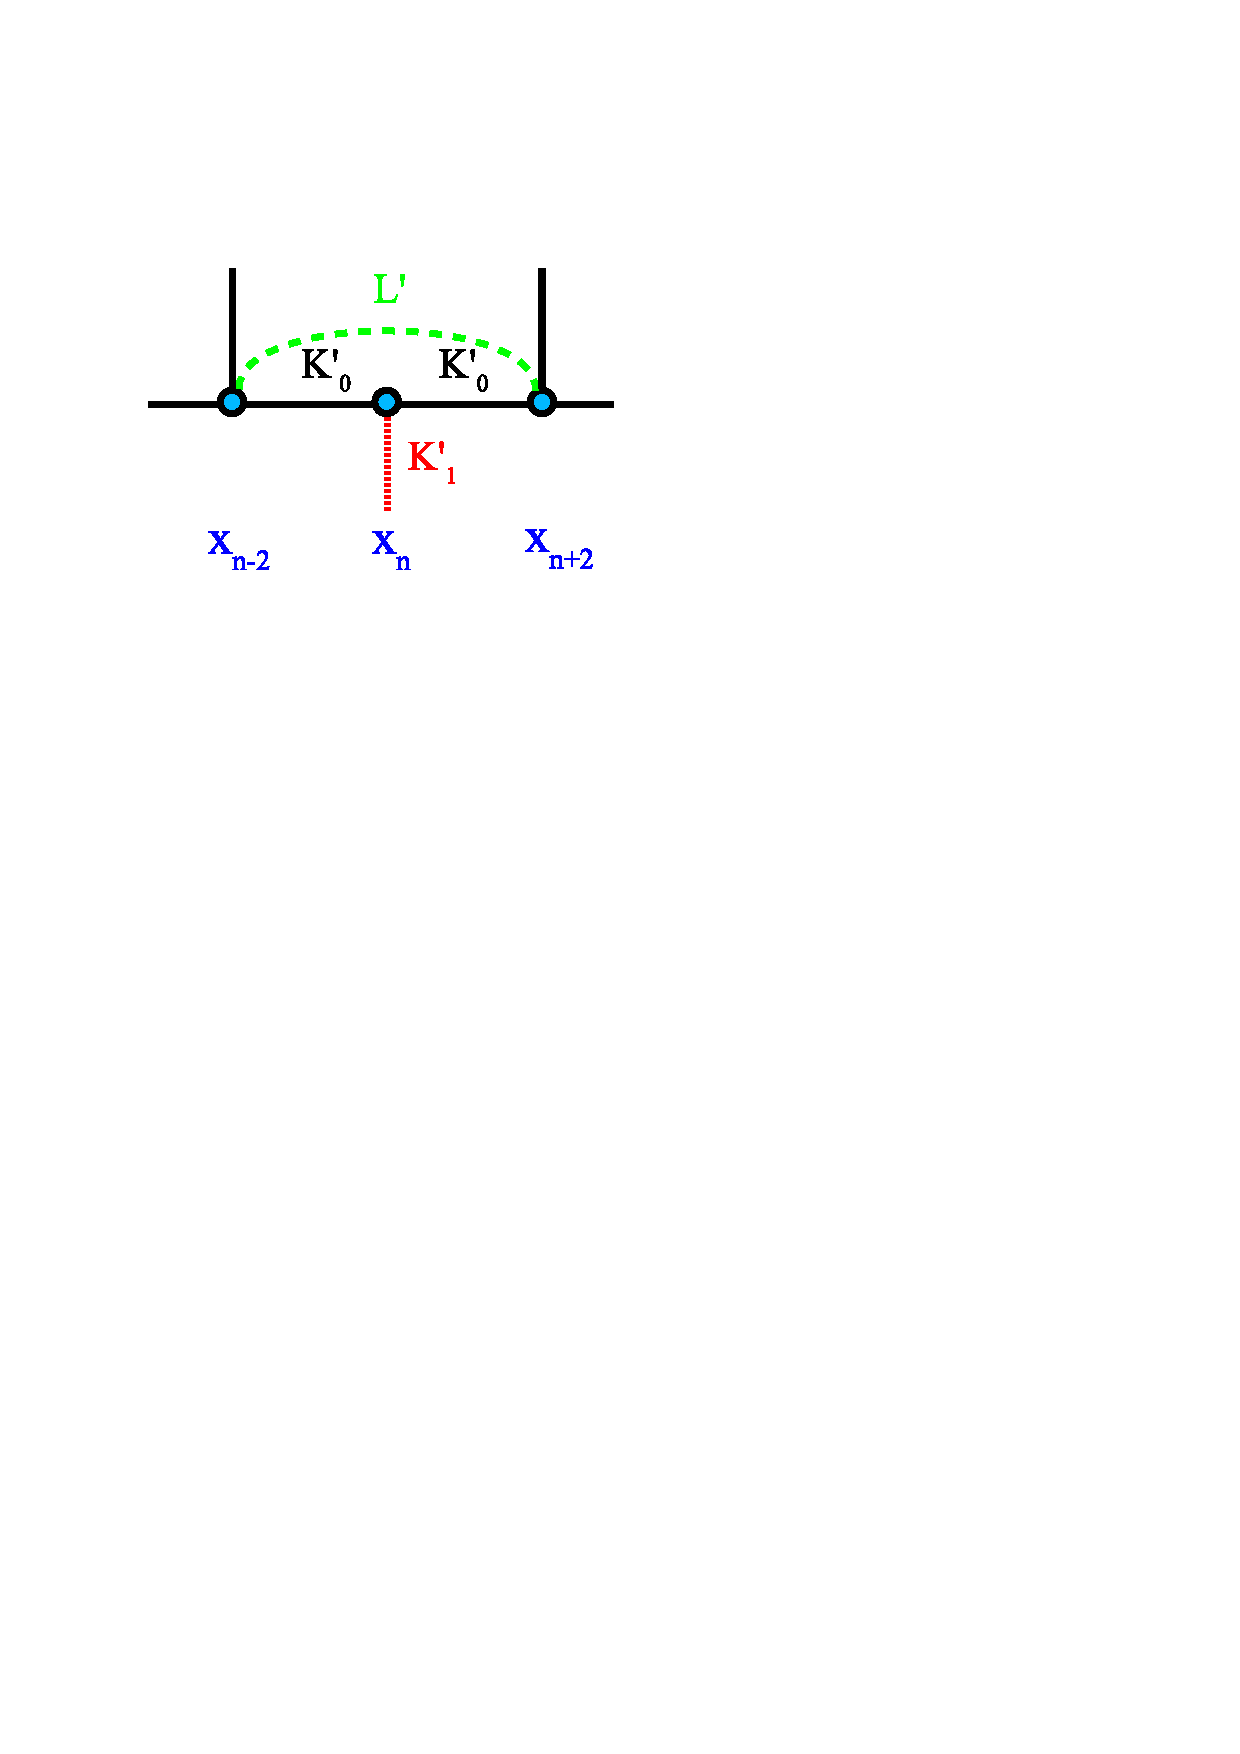
\includegraphics[scale=0.68]{Chapter-3/RG3hanoi_after}
\protect\caption{Hanoi networks three-spin graph after tracing over $x_{n\pm 1}$.}
\label{fig:afm-hn3rgafter} 
\end{figure}

After tracing over the odd spins $x_{n\pm 1}$, the long-range coupling as well the $K_0$ and $L$ between low-level sites is renormalized into $K_0 '$ and $L'$. The depiction of the graph left is shown in Fig. \ref{fig:afm-hn3rgafter} \cite{Boettcher2011HNNP}, which is about {\it half} of  Fig. \ref{fig:afm-hn3rgbefore} \cite{Boettcher2011HNNP}. $K_1 '$ in Fig. \ref{fig:afm-hn3rgafter} \cite{Boettcher2011HNNP} connects to another adjecent {\it half}, which produces another five-spin RG unit. By recursively renormaling the graph, the system size is reduced exponentially, and the final graph simply has 3 spins but very complicated couplings $K_0 ', K_1 ' $ and $L'$. The most important part in RG is to calculate these renormalized couplings.


\begin{figure}
\centering 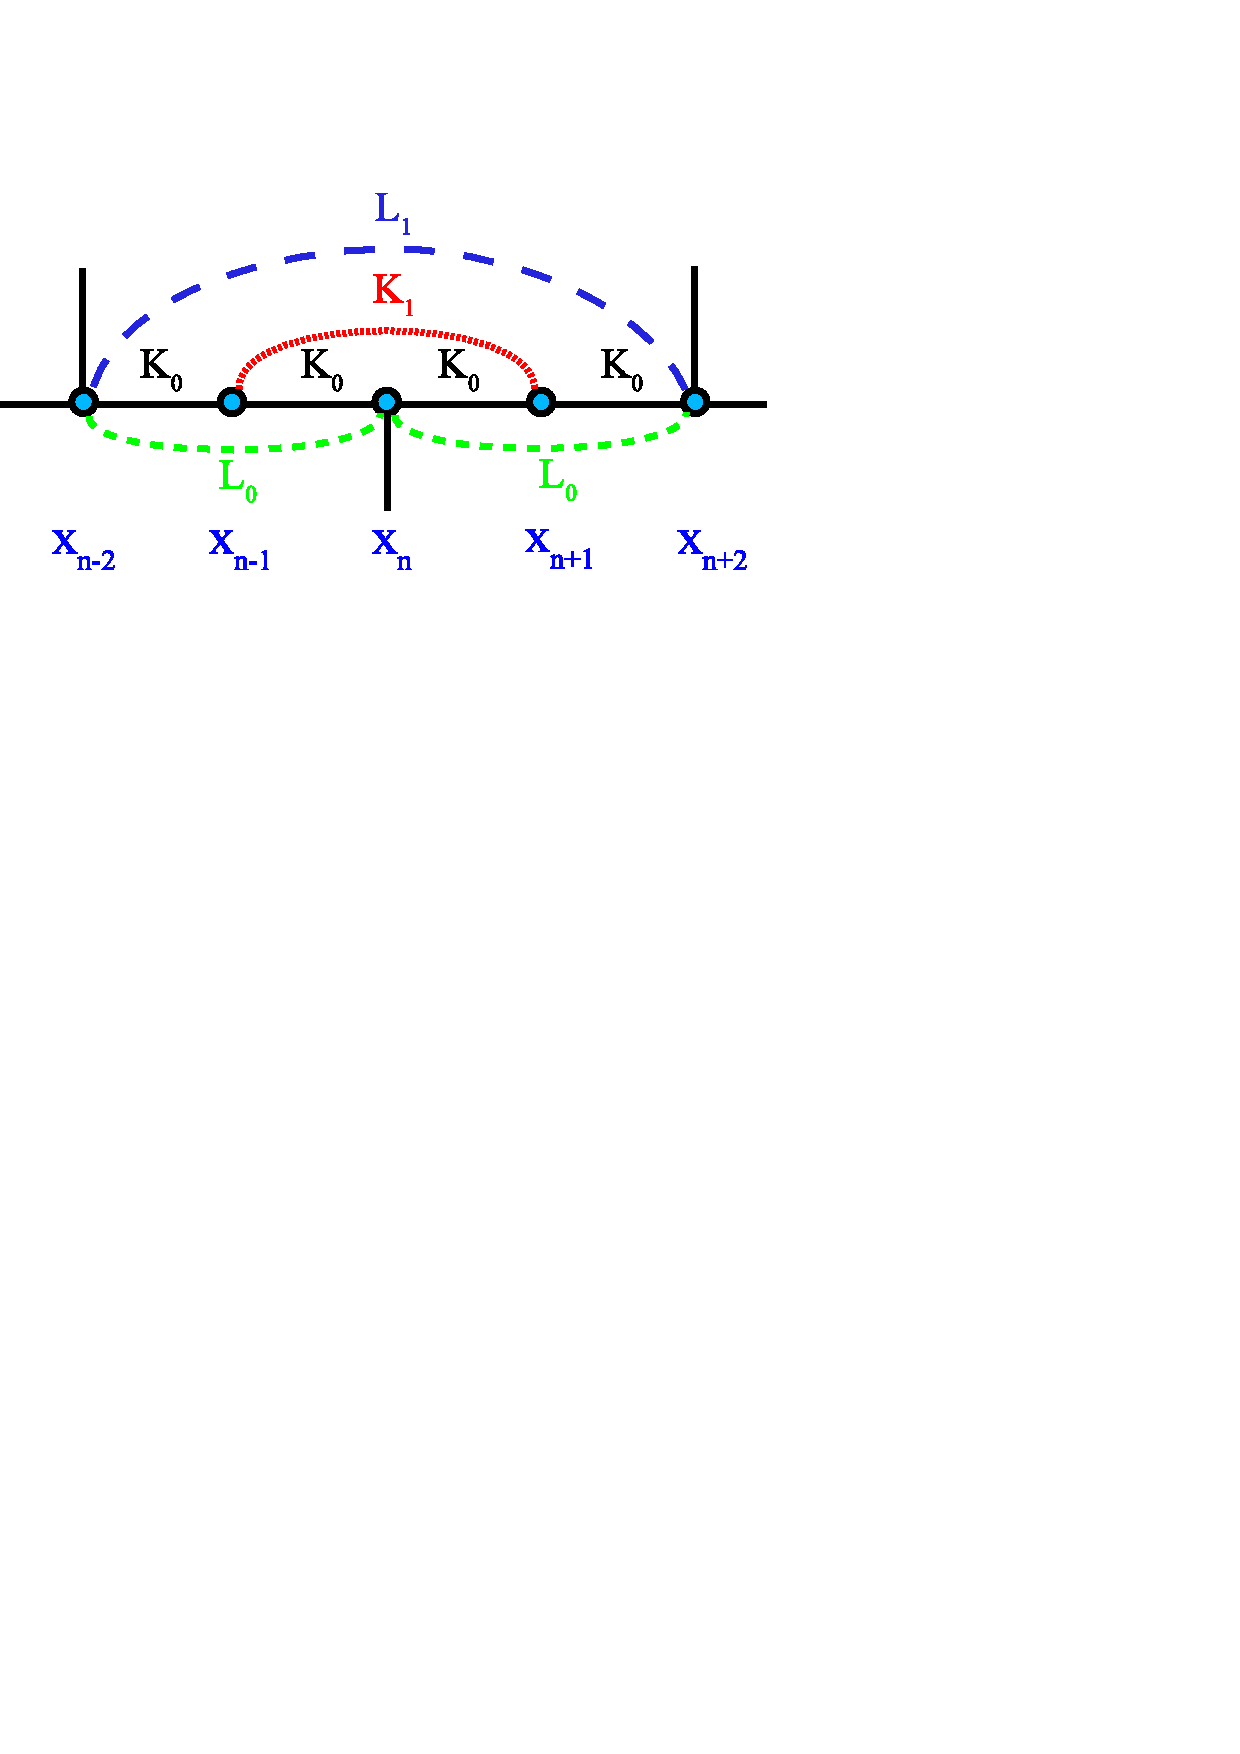
\includegraphics[scale=0.68]{Chapter-3/IsingRG_HN5_before}
\protect\caption{HN5 five-spin RG unit with all the couplings among the spins.}
\label{fig:afm-hn5rg} 
\end{figure}

\begin{figure}
\centering 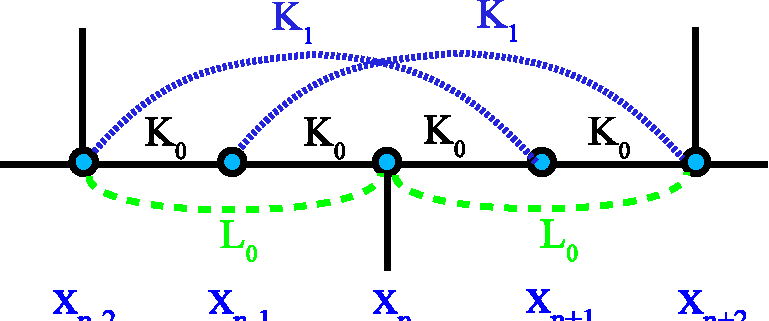
\includegraphics[scale=0.68]{Chapter-3/IsingRG_HNNP_before}
\protect\caption{HNNP five-spin RG unit with all the couplings among the spins.}
\label{fig:afm-hnnprg} 
\end{figure}

\begin{figure}
\centering 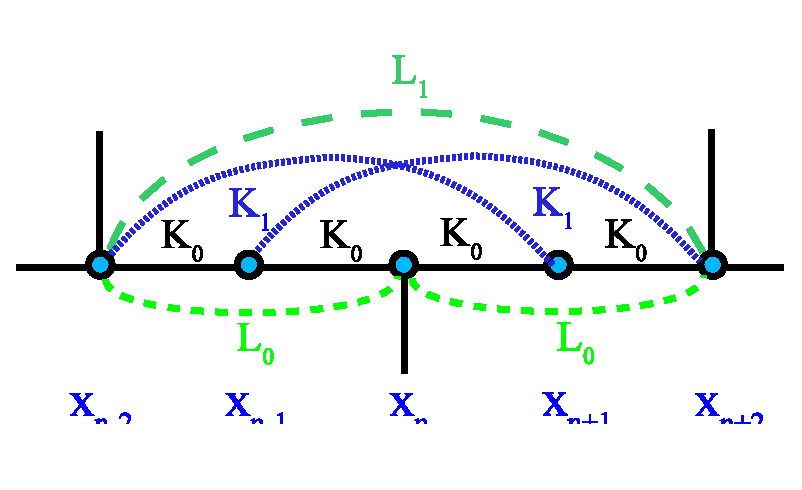
\includegraphics[scale=0.68]{Chapter-3/IsingRG_HN6_before}
\protect\caption{HN6 five-spin RG unit with all the couplings among the spins. $L_1$ is another interaction term emerging in the RG steps.}
\label{fig:afm-hn6rg}
\end{figure}

In addition to HN3, the other three networks have different setup of the five-spin RG unit but the same three-spin renormalized RG graph. The 5-spin graphlets are shown in Fig. \ref{fig:afm-hn5rg} \cite{Boettcher2011HNNP} for HN5, in Fig. \ref{fig:afm-hnnprg}  \cite{Boettcher2011HNNP} for HNNP, and in Fig. \ref{fig:afm-hn6rg} \cite{Boettcher2011HNNP} for HN6. 



\subsection{RG without magnetic fields}
The setup of RG is started by separating the AFM's Hamiltonian into hierarchies
\begin{equation}
-\beta\mathcal{H} = \sum_{n=1}^{k-2} (-\beta \mathcal{H}_n)+ \mathcal{R}(K_2, K_3, \cdots)
\end{equation}
where $\mathcal{R}$ is the coupling beyond $\mathcal{H}_n$ of levels $k>2$. $\mathcal{H}_n$ depends on the interactions $K_0$ on the backbone and $L_0$, $L_1$, $K_1, \cdots$ among the long range couplings. The detailed RG procedure is described network by network. 

\subsubsection{HN3, HN5, and their interpolations }
\label{sec:afm-HN35RG}

For HN3 and HN5, the Hamiltonian $\mathcal{H}_n$ for each hierarchy with 5 Ising spins is
\begin{eqnarray}
\label{eq:hn35-z0}
 -\beta \mathcal{H}_n &=& K_0 \left(x_{n-2}x_{n-1} + x_{n-1}x_{n} +  x_{n}x_{n+1} +  x_{n+1}x_{n+2}\right) \nonumber \\ 
   && + K_1(x_{n-1}x_{n+1}) + L_0(x_{n-2}x_{n} + x_{n}x_{n+2}) \nonumber \\
   && + y L_1 (x_{n-2} x_{n+2})  + 4I 
\end{eqnarray}
where $y$ is 0 for HN3 and 1 for HN5. $y$ can be extended to a wide range of parameters from $-\infty$ to $+\infty$, which leads to the interpolations of HN3 and HN5. These interpolations may introduce more interesting phases and transitions. $K_0$ is the interaction term of the 1D backbone. In terms of traditional Ising model's interaction term $J_0$, $K_0=\beta J_0$ which is usually $\beta=-1/T$ by setting $J_0=-1$ for AFM. The long range links over the same hierarchies have the coupling term $K_1$ ($=\beta J_0$) which is set as a constant in this RG flow. $L_0$ also stands for the coupling term emerged in the RG flow, and its initial value is 0. $L_1$ is accounted for the extra long range links in HN5 comparing to HN3. The last term $I$ is a constant emerging after the first step of RG, and its initial value is 0. Its coefficient $4$ is a simply a mathematical choice because there are effectively 4 spins in each hierarchy. The \underline{\emph{initial values}} for these parameters are
\begin{equation}
\begin{array}{l}
\displaystyle I = 0 \\
\displaystyle K_0 =\beta J_0=-\frac{1}{T} < 0 \\
\displaystyle K_1 =\beta J_0=-\frac{1}{T}  < 0 \\
\displaystyle L_0 = 0 \\
\displaystyle L_1 =\beta J_0 =-\frac{1}{T} < 0 \\
\end{array} 
\label{eq:hn35-init1}
\end{equation}
where Boltzmann constant $k$ is set as 1 here. $K_1$ is not changing in the RG flow because it is introduced again at every RG step. Therefore, it is equivalent to $-1/T$ which can be used as a reference to temperature. High temperatures $T \rightarrow \infty$ stands for $K_1\rightarrow -0$; while low temperatures $T\rightarrow 0$ corresponds to large $K_1 \rightarrow -\infty$.

After tracing over the sites $x_{n-1}$ and $x_{n+1}$, we can get this form of equation
\begin{equation}
\label{eq:hn35-z1}
 -\beta \mathcal{H}_n = 2I' +  K'_0 \left(x_{n-2}x_{n} +  x_{n}x_{n+2}\right) + L'_0(x_{n-2}x_{n+2})
 \end{equation}
 which is `half' of original RG setup.
For the convenience of mathematical and computational analysis, these parameters is transformed to a new set of activity parameters  
\begin{equation}
\begin{array}{l}
\displaystyle C = e^{-4I}   \\
\displaystyle \kappa = e^{-4K_0} \\
\displaystyle \lambda = e^{-4L_0}  \\
\displaystyle \mu = e^{-2K_1} = e^{-2L_1} 
\end{array} 
\label{eq:hn35-activities}
\end{equation}
The pre-factors of $K_0, K_1, I ,$ and $ L_1$ is for the convenience of the RG calculations. Thus, the  new \underline{\emph{initial values}}  are


\begin{equation}
C = 1,   \kappa = \mu^2 > 1, \lambda =\mu^{2y} , \mu >1 
\label{eq:hn35-init1}
\end{equation}
where $\mu$ is equal to $e^{2/T}$ since $K_1$ is set as a constant of $-1/T$. Apparently, only $\mu$ needs to be specified to start the numerical RG flow. In other words, the initial values for HN3($y=0$) and HN5($y=1$) are determined by $\mu$ and $y$.

To establish an intuitive connection to these defined RG parameters, the relationship between $\mu$ and $T$ is ,  
\begin{equation}
\begin{array}{l}
\displaystyle T\rightarrow 0 \ \Leftrightarrow \ \ K_1 \rightarrow -\infty  \ \Leftrightarrow \ \ \mu \rightarrow \infty   \ \Leftrightarrow  \ \ {1}/{\mu}\rightarrow 0+\\
\displaystyle T\rightarrow \infty  \ \Leftrightarrow  \ K_1 \rightarrow 0- \ \Leftrightarrow  \ \ \mu \rightarrow 1+ \  \ \Leftrightarrow  \ \  {1}/{\mu}\rightarrow 1- \\
\end{array} 
\label{eq:Ts}
\end{equation}
, and the relationship among $\kappa$, $J_0$, temperature $T$, and $\mu$ is
\begin{equation}
\begin{array}{l}
J^{(0)} = -1,  \\ 
T = 2/\log(\mu) \\ 
J^{(n)} = -\frac{T}{4}\log\kappa^{(n)} \\
\end{array}
\label{eq:afm-hn35-jk}
\end{equation} 
where $J^{(0)}$ stands for the initial value in the RG flow and is the same as $J_0$, and $J^{(n)}$ and $\kappa ^{(n)}$ are the $i$-th renormalized variables.

By tracing over all the $\{x_n\}$ in Eq. \ref{eq:hn35-z0} and Eq. \ref{eq:hn35-z1}, we can get $2^{3}$ equations with 3 unknown variables ($ K_0,  L_0, I$). The solutions in terms of $(\kappa, \lambda, C)$ are
\begin{equation}
\begin{array}{l}
\displaystyle \kappa' = \frac{2\kappa \lambda (1+\mu) }{\kappa^2+2\mu \kappa +1} \\
\\
\displaystyle \lambda' = \mu^{2y} \frac{(1+\mu)(1+\kappa)^2}{2(\kappa^2+2\mu \kappa +1)}\\ \\
\displaystyle C' =  \frac{C^2 \kappa\mu}{\sqrt{2} (1+\kappa) (1+\mu)^{3/2}  \sqrt{ \kappa^2+2\mu \kappa +1}}   \\
\end{array} 
\label{eq:afm-hn35sol1}
\end{equation}

These solutions are the same as the RG process in FM Ising model \cite{Boettcher2011HNNP}, but the RG results afterward are very different due to the inherent frustrations and complexity in AFM. The fixed point analysis is continued in Sec. \ref{sec:afm-results}.



\subsubsection{ HNNP, HN6, and their interpolations }
The initial RG setup of planar networks, HN3 and HN5, has been described in the previous subsection. While the non-planar networks, HNNP and HN6, share a similar setup except for different interaction terms due to different long-range links in these small-world networks. The $\mathcal{H}_n$ for each hierarchy is 
\begin{eqnarray}
 -\beta \mathcal{H}_n &=& K_0 \left(x_{n-2}x_{n-1} + x_{n-1}x_{n} +  x_{n}x_{n+1} +  x_{n+1}x_{n+2}\right) \nonumber \\ 
   && + K_1(x_{n-2}x_{n+1} + x_{n-1}x_{n+2}) + yL_1(x_{n-2} x_{n+2}) \nonumber \\
   && +L_0(x_{n-2}x_{n} + x_{n}x_{n+2})  + 4I 
\label{eq:hp-z0}
\end{eqnarray}
where $y$ is 0 for HNNP and 1 for HN6. The interpolations of HNNP and HN6 can also be easily explored using different $y$'s. $K_0$ ($=\beta J_0= -1/T$) is the interaction term of the 1D backbone. $K_1$ ($=\beta J_0$) is also set as a constant $\beta J_0$ ($=-1/T$). $L_0$ is an emerging terms after the first RG step, and $L_1$ is for the extra long range links in HN6 comparing to HNNP. $I$ is still a constant. The \underline{\emph{initial values}} for these parameters are All the initials values for these activity parameters are
\begin{equation}
\begin{array}{l}
\displaystyle I = 0 \\
\displaystyle K_0 =\beta J_0=-\frac{1}{T} < 0 \\
\displaystyle K_1 =\beta J_0=-\frac{1}{T}  < 0 \\
\displaystyle L_0 = 0 \\
\displaystyle L_1 =\beta J_0 =-\frac{1}{T} < 0 \\
\end{array} 
\label{eq:hp-init1}
\end{equation}

By tracing the sites $x_{n-1}$ and $x_{n+1}$, the reduced form of Hamiltonian with 3 spins is
\begin{equation}
\label{eq:hnnpz1}
 -\beta \mathcal{H}_n = 2I' +  K'_0 \left(x_{n-2}x_{n} +  x_{n}x_{n+2}\right) + L'_0(x_{n-2}x_{n+2})
 \end{equation}
 which is the same as that in HN3 and HN5. Similarly, a new set of parameters is introduced, and their definitions and possible values are  
 \begin{equation}
\begin{array}{l}
\displaystyle C = e^{-4I} > 0   \\
\displaystyle \mu = e^{-2K_1} = e^{-2L_1} > 1 \\
\displaystyle \kappa = e^{-4K_0} > 1 \\
\displaystyle \lambda = e^{-4L_0}  > 1\\
\end{array} 
\label{eq:hn35-activities}
\end{equation}
Their corresponding initial values are 
 \begin{equation}
 C = 1,  \kappa = \mu^2,  \lambda =  \mu^{2y} 
\label{eq:hp-init2}
\end{equation}
where $y$ can be 0 for HNNP, 1 for HN6, and any other values for thier interpolations. All the initials values for these activity parameters are the same as in HNNP. The RG recursive equations are
\begin{equation}
\begin{array}{l}
\displaystyle \kappa' = \frac{\kappa \lambda (1+\mu)^2 }{(1+\mu\kappa)^2} \\
\\
\displaystyle \lambda' =\mu^{2y} \frac{(\kappa + \mu)^2} {(1 + \mu \kappa)^2} \\ \\
\displaystyle C' =  \frac{C^2 \kappa\mu^2} {(1+\mu)^2 (\kappa+\mu) (1+ \mu\kappa)}   \\
\end{array} 
\label{eq:afm-hpsol1}
\end{equation}
These solutions are also the same as those in Ref. \cite{Boettcher2011HNNP}, but we expect possible glassy and chaotic behaviors introduced in AFM and these complex networks.


\subsection{RG with magnetic fileds}
In order to study a broad range of physical properties using RG, the external magnetic field $H$ is needed. We plan to explore different physical properties, such as internal energy $e$, magnetization $m$, free energy $f$, entropy $s$, specific heat $c_v$, and magnetic susceptibility $\chi$. 

Here the RG setup is extended to a more general scenario by including $H$. The procedure of such RG has been developed by Brunson and Boettcher in FM of Hanoi networks \cite{brunson2014rg}. In AFM, the same procedure is followed with corresponding adjustments of temperature $T$ ($\mu$ in RG) and prefactors of these derivations. Instead of detailed derivations \cite{brunson2014rg}, only the general logic and the formulations of targeted physics properties are described in this section. 

The starting point of all these equilibrium physical properties is the partition function $Z$. As shown in Fig. \ref{fig:afm-hn3rgafter}, the partition function of the smallest system size $N=2^1+1=3$
\begin{equation}
Z^{(1)} = e^{-\beta \mathcal{H} ( K^{(1)}, L^{(1)}, \cdots ;\  x_1, x_2, x_3)}
\end{equation}
where $K^{(1)}, L^{(1)}, \cdots$ stands for the raw activity parameters of temperature $T$, coupling $J$, and magnetic field $H$; $x_1, x_2$, and $ x_3$ are the 3 spins ($\pm 1$). 
Using RG and its recursive solutions (similar to Eq. \ref{eq:afm-hn35sol1} in RG without magnetic field), it is easy to obtain the renormalized activity parameters  $K^{(n)}, L^{(n)}, \cdots$. The superscript $n$ means system size $N=2^n + 1$. 

The physical properties calculated are
\begin{enumerate}
\item internal energy per spin
\begin{equation}
e = -\frac{1}{N}\frac{\partial \ln Z}{\partial \beta}
\end{equation}
The goal is to find the equilibrium energy to uncover the non-equilibrium dynamics in simulations.

\item Free energy per spin
\begin{equation}
f = - \frac{1}{N}\frac{1}{\beta} \ln Z
\label{eq:afm-free}
\end{equation}

\item Free energy difference between parallel and anti-parallel boundary conditions

The equation of the free energies is still the same as Eq. \ref{eq:afm-free}. The difference is that the first spin ($x_0$) and last one ($x_{N}$) are fixed, i.e., the parallel boundary condition ($f_1$) have both $x_0 = x_N = +1$, while the anti-parallel boundary condition ($f_2$) has $x_0=+1$ but $x_N=-1$. The difference is
\begin{equation}
\Delta f = f_1 - f_2 = - \frac{1}{N}\frac{1}{\beta} ( \ln Z_{++} - \ln Z_{+-}) =- \frac{1}{N}\frac{1}{\beta}  \ln \frac{Z_{++}}{ Z_{+-}}
\label{eq:afm-freediff}
\end{equation}
where $Z_{++}$ and $Z_{+-}$ stand for the partition functions of parallel and anti-parallel boundary conditions, respectively.

The goal of this parameter is to discover the chaotic dynamics and spin glass phase. In a spin glass system with chaotic dynamics, the difference $\Delta F$ is non-zero in the thermodynamic limit and changes signs at different temperatures \cite{wang2015chaos}. In a range of temperatures, the number of times of changing sign of $\Delta F$ may increase  with system size following a power-law. 

\item entropy per spin
\begin{equation}
s = \frac{1}{N} \frac{\partial}{\partial T} \left( \frac{1}{\beta} \ln Z \right)
\end{equation}
Entropy may be useful to understand the geometric frustrations and compared to Wang-Landu sampling's density of states. 

\item magnetization per spin
\begin{equation}
m = \frac{1}{N}\frac{1}{\beta} \frac{\partial \ln Z}{\partial H}
\end{equation}
The magnetization may have interesting patterns at low temperatures \cite{ohanyan2003mag, kageyama2000direct} due to complex local spin configurations.

\item specific heat per spin
\begin{equation}
c_v = \frac{\partial e} {\partial T}
\end{equation}
If there is any second-order phase transition, specific heat $c_v$ may show the transition.

\item magnetic susceptibility per spin
\begin{equation}
\chi = \frac{\partial m} {\partial H}
\end{equation}
If there is any second-order phase transition, susceptibility  $c_v$ may show the transition.

\end{enumerate}

There equations are trivial and can be found in the textbook, but their implementation in RG take a large amount of analytical deviations and numerical testing. The detailed description can be found in the work by Brunson and Boettcher \cite{brunson2014rg}.


\section{Results}
\label{sec:afm-results}
The most common observations in AFM with geometric frustraions are the glassy dynamics at low temperatures, which is often observed in experiments and simulations. However, the equlibrium behaviors near and beyond the critical point can only be detected using analytical method. Using both the computational and analytical methods introduced the previous section, results of dynamic properties, fixed point analysis, and corresponding equlibrium properties are described in Sec. \ref{sec:afm-dyn}, Sec. \ref{sec:afm-fpa}, and Sec. \ref{sec:afm-eqa}, respectively.

\subsection{Dynamic Properties}
\label{sec:afm-dyn}
The interesting glassy dynamics can be observed from simulational experiments using simulated annealing described in Sec. \ref{sec:afm-mc}. In the simulations, the only control parameter is the temperature $T$. The starting point is high $T$ ($T=10.0$) which corresponds to 
 paramagnetic disordered states. As the $T$ is decreased, the system is more and more likely to
 accept a transition to a lower energy state. In a system with no geometric frustrations, a low $T\rightarrow0$ would lead to the ground state with the lowest energy. However, AFM in Hanoi networks cannot reach ground states due to complex geometric frustrations. 

\begin{figure}
\centering 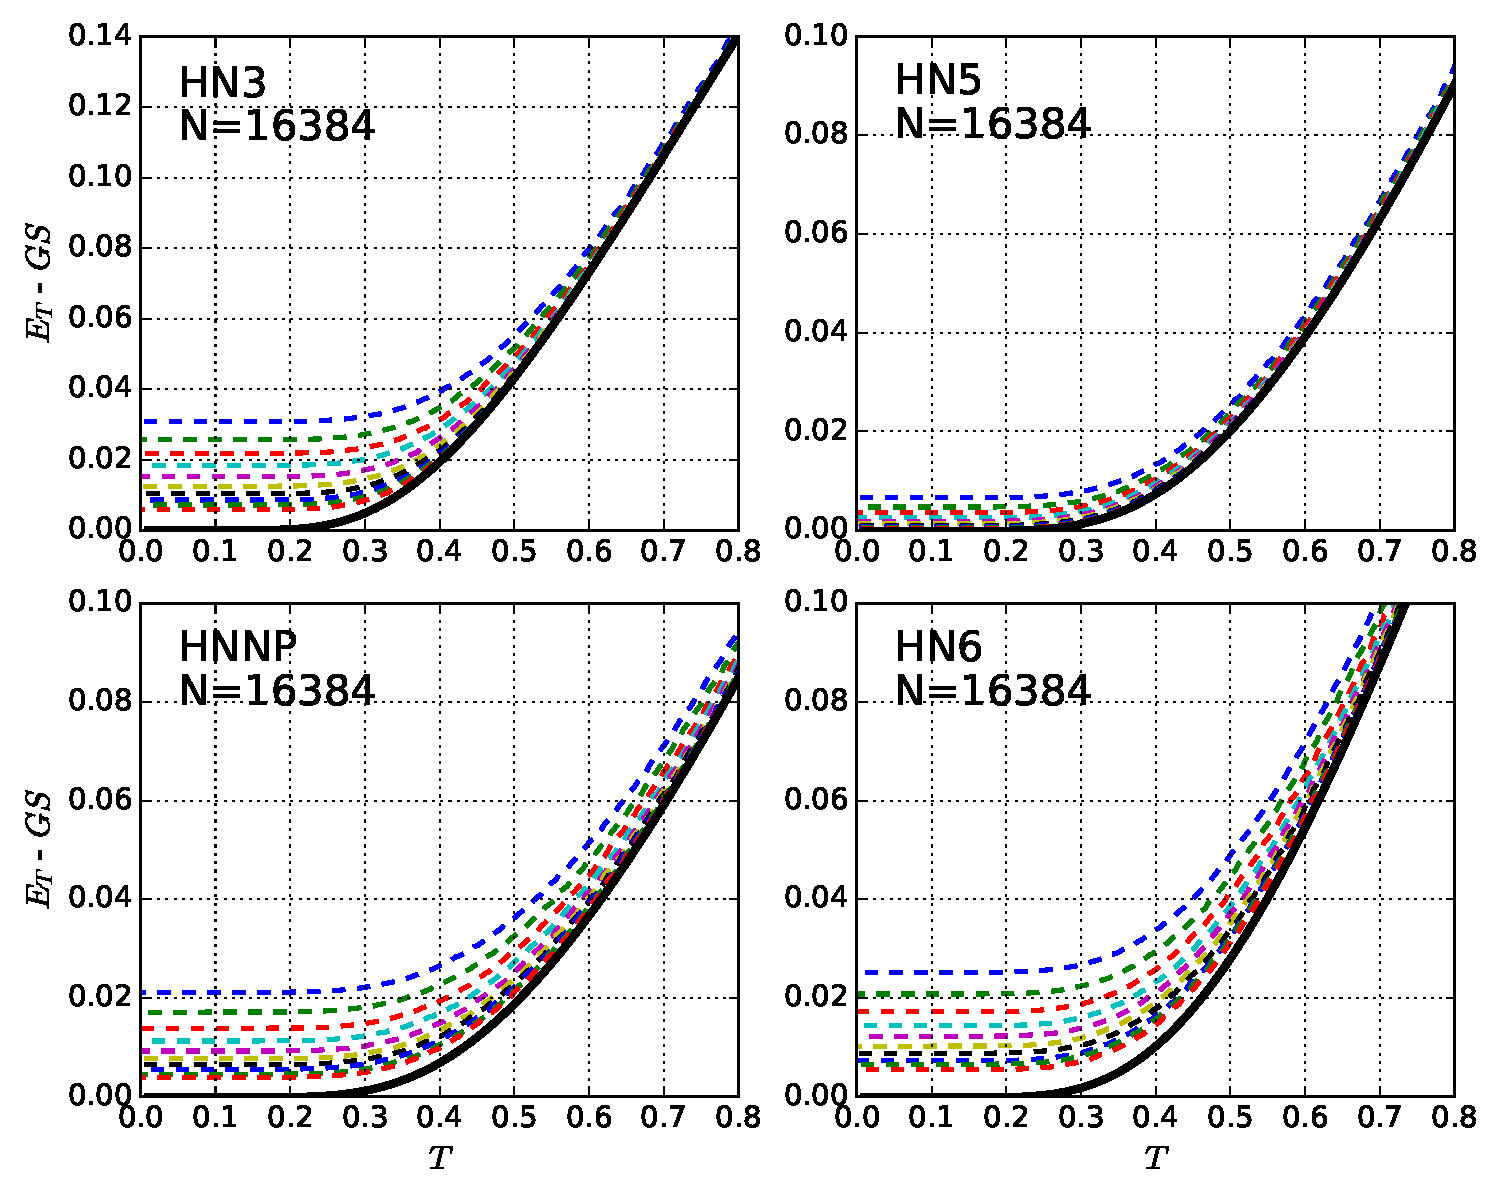
\includegraphics[width=0.9\columnwidth]{Chapter-3/AFM_Jamming_SA_plot}
\protect\caption{Energy vs. temperature $T$ from the Simulated Annealing of all the four networks. In each of the 4 subfigures, the dotted curves from top to bottom correspond to annealing schedules of $10^{-3},  10^{-3}/2^1, 10^{-3}/2^2, \cdots, 10^{-3}/2^9$, respectively. The slowest annealing schedule is $1.95\times10^{-6}$. The solid black curves on the bottom are the equilibrium curves from RG, which clearly shows the gap between equilibrium and non-equilibrium behaviors.}
\label{fig:afm-hnsjam} 
\end{figure}

The behavior at low $T$ is similar to what is observed in the jamming systems in Chapter \ref{chap-jamming}. As shown in Fig. \ref{fig:afm-hnsjam} and \ref{fig:afm-hnsscaling}, all four
 networks show the glassy dynamics with a power relaxation. HN5 may reach equilibrium ground
 states at a much slower annealing schedules due to increasing variations at lower schedules. Other networks have clearly a gap between 'jammed' state and the equilibrium ground states, and the gap can only be eliminated at an infinitely slow annealing rate after an infinitely long time due to the power-law scaling.

\begin{figure}
\centering 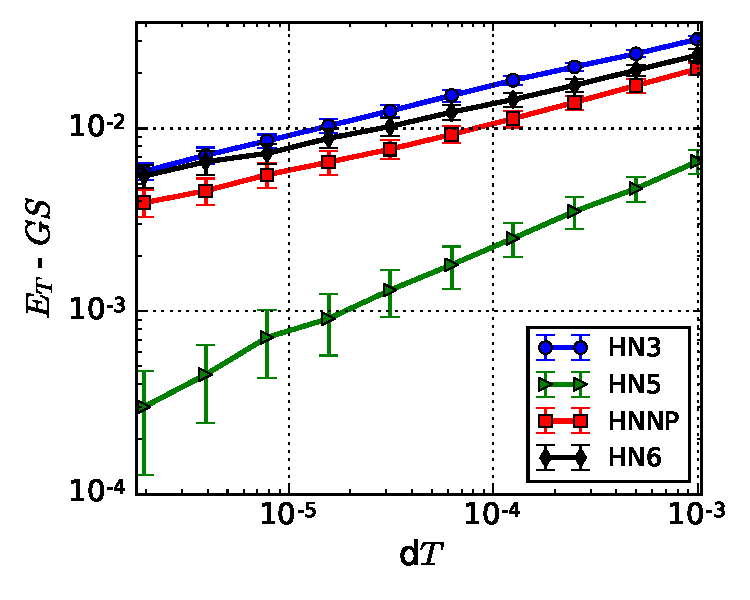
\includegraphics[width=0.5\columnwidth]{Chapter-3/AFM_Jamming_SA_scaling_plot}
\protect\caption{Scaling of  dynamically reached lowest energy at different annealing schedules. The error bar is calculated from $100$ or more runs with different random initializations. The ground states are obtained using renormalization group.}
\label{fig:afm-hnsscaling} 
\end{figure}

In order to get the relaxation scaling in Fig. \ref{fig:afm-hnsscaling}, the most challenging part is to find the ground states. Unlike the exact and fractal "ground states" in the jamming systems, AFM in these four HNs has different but converging ground states as the system size gets larger and larger. Wang-Landu sampling fails to produce ground states for system sizes $N>2^{10}$, and renormalization group (RG) has to be used to find the ground states at different system sizes. From RG calculations, the equilibrium ground states for HN3, HN5, HNNP, and HN5 at system size $N=2^{14}$ are $-1.0$, $-1.166503...$, $-1.480224...$, $-1.285644...$, respectively.  More details of  RG and equilibrium properties are discussed in Sec. \ref{sec:afm-eqa}.

\subsection{Fixed Point Analysis}
\label{sec:afm-fpa}
Starting from the recursive solutions of Eq. \ref{eq:afm-hn35sol1} and Eq. \ref{eq:afm-hpsol1} in Sec. \ref{sec:afm-rg}, the fixed point analysis can help discover possible chaotic and critical behaviors. 

\subsubsection{ HN3, HN5, and their interpolations }
For HN3 with $y=0$ in Eq. \ref{eq:afm-hn35sol1}, there are 2 analytical fixed points which are
\begin{equation}
\displaystyle \kappa^* = 1, \lambda^* =1; 
\label{eq:afm-fps3-1}
\end{equation}
\begin{equation}
\displaystyle \kappa^* = 0, \lambda^* =\frac{1+\mu}{2} 
\label{eq:afm-fps3-2}
\end{equation}
where only the first one is a stable fixed point solution. The second one is only stable at the high temperature limit, and any finite temperatures lead to the fixed point $\kappa^* =1, \lambda^* = 1.$ The stability of the two fixed points is mathemtically analyzed using the Jacobian matrix later in this section.

HN5 with $y=1$ has more interesting fixed points are more interesting. The two fixed point solution are
\begin{equation}
\kappa^* = 0, \ \  \lambda^* = \mu^{2y}\frac{\mu+1}{2}
\label{eq:afm-fps5-1}
\end{equation}

\begin{equation}
\begin{array}{l}
\displaystyle \kappa^* = \frac{1}{2}\left[\mu^2 -\mu + \sqrt{(\mu+1)(\mu^3 - 3\mu^2 +8\mu-4)} \right]  \\  \\
\displaystyle \lambda^* = \frac{\mu}{4}\left[\mu^2 -\mu+2 + \sqrt{(\mu+1)(\mu^3 - 3\mu^2 +8\mu-4)} \right]
\end{array} 
\label{eq:afm-fps5-2}
\end{equation}

With different $y$,  the parameter of interest $\kappa$ in Eq. \ref{eq:afm-fps5-2} can be written in a general form as a function of $\mu$ ($\mu>1$) and $y$
\begin{equation}
\kappa^* = \frac{1}{2}\Big[\sqrt{4\left( \mu^{1+y} + \mu^{y} - 1\right)+\left( \mu^{1+y} + \mu^{y} - 2\mu\right)^2}+ 
\mu^{1+y}+\mu^{y} -2\mu \Big] 
\label{eq:afm-fyps_k}
\end{equation}
, and the corresponding $\lambda$ is
\begin{equation}
\lambda^* = \frac{\mu ^y}{4}  \left(2 \mu +\mu ^{y+1}+\mu ^y-\sqrt{(\mu +1) \left(4 \mu +\mu ^{2 y}+4 \mu ^{y+1}+\mu ^{2 y+1}-4 \mu ^y-4\right)}-2\right)
\label{eq:afm-fyps_l}
\end{equation}

The stability of the fixed points can be proved by both numerical iterations (as shown in Fig. \ref{fig:afm-HN35KJ_ys}) and the eigenvalue of the Jacobian from Eq. \ref{eq:afm-hn35sol1}. The Jacobian matrix is
\begin{equation}
  Jacobian(\kappa,\lambda; \mu) =
\left(\frac{\partial(\kappa', \lambda')}{\partial(\kappa, \lambda)}\right)=
\left( {\begin{array}{*{50}c}
J_{11} & J_{12}\\
J_{21} & J_{22}
 \end{array} } \right)
=
\left( {\begin{array}{*{50}c}
\frac{\partial \kappa'}{\partial \kappa}&\frac{\partial \kappa'}{\partial \lambda}\\
\frac{\partial \lambda'}{\partial \kappa}&\frac{\partial \lambda'}{\partial \lambda}\\
 \end{array} } \right)
\label{eq:hn35-j}
\end{equation}
where $Jacobian$ is used to avoid conflicts with the interaction constant $J$, and the matrix elements are
\begin{equation}
J_{11} = \frac{\partial \kappa'(\kappa, \lambda)}{\partial \kappa}=-\frac{2 (\kappa -1) (\kappa +1) \lambda  (\mu +1)}{\left(\kappa ^2+2 \kappa  \mu +1\right)^2}
\end{equation}
\begin{equation}
J_{12} =  \frac{\partial \kappa'(\kappa, \lambda)}{\partial \lambda}= \frac{2 \kappa  (\mu +1)}{\kappa ^2+2 \kappa  \mu +1}
\end{equation}
\begin{equation}
J_{21} =\frac{\partial \lambda'(\kappa)}{\partial \kappa}=\frac{(\kappa -1) (\kappa +1) (\mu -1) (\mu +1) \mu ^{2 y}}{\left(\kappa ^2+2 \kappa  \mu +1\right)^2}
\end{equation}
\begin{equation}
J_{22} = \frac{\partial \lambda'(\kappa)}{\partial \lambda}=0
\end{equation}

From the Jacobian matrix, it is easy to calculate the eigenvalues which is not shown here due to its complex and long form. The fixed points of Eq. \ref{eq:afm-fyps_k} and Eq. \ref{eq:afm-fyps_l} produce eigenvalue with magnitude less than 1, which means stable fixed points.

\begin{figure}
\centering 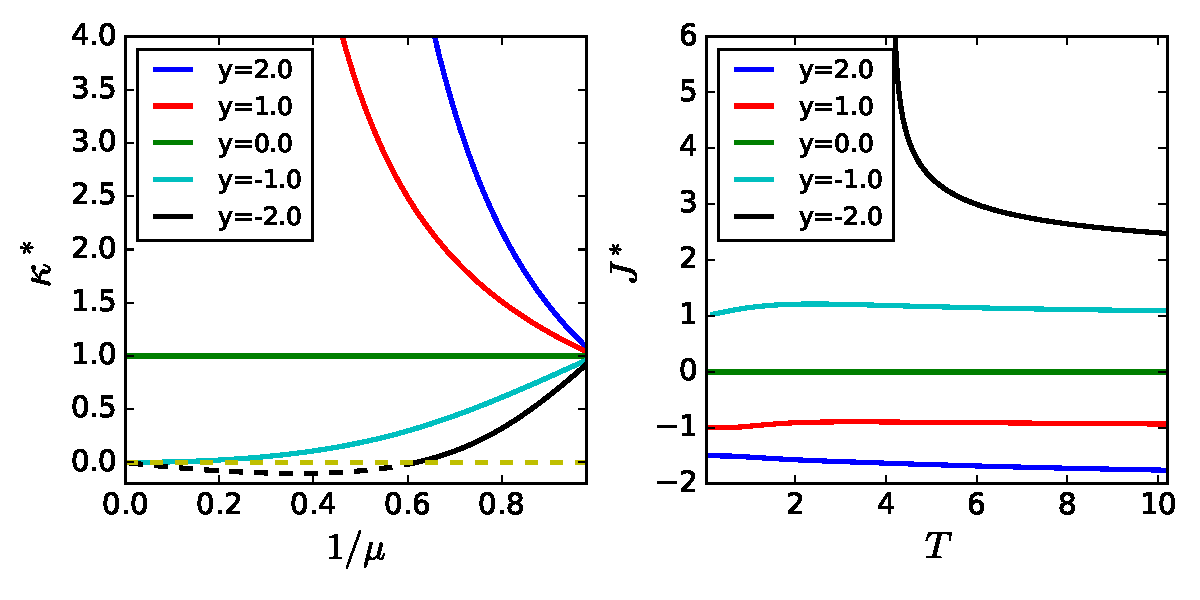
\includegraphics[width=0.9\columnwidth]{Chapter-3/HN35_KJvsTys.pdf}
\protect\caption{The numerical fixed points of $\kappa^*$ and corresponding $J^*$ using Eq. \ref{eq:afm-hn35-jk2} for HN3, HN5, and their interpolations. $y=0$ corresponds to HN3; $y=1$ corresponds to HN5; and $y<0$ corresponds that the extra bonds of HN5 comparing to HN3 are ferromagnetic. }
\label{fig:afm-HN35KJ_ys} 
\end{figure}


The fixed point as a function of temperature ($\mu$ or $T$) at different $y$'s are shown in Fig. \ref{fig:afm-HN35KJ_ys}. Equivalently, the fixed point of $\kappa^*$ is the converged renormalized $\kappa^*$ , and the corresponding interaction constant $J^*$ is the renormalized interaction constant in the thermodynamic limit. Based on Eq. \ref{eq:afm-hn35-jk}, the relationship between $\kappa^*$ and $J^*$ is
\begin{equation}
J^* = -\frac{T}{4} \log \kappa^*
\label{eq:afm-hn35-jk2}
\end{equation}




\begin{figure}
\centering 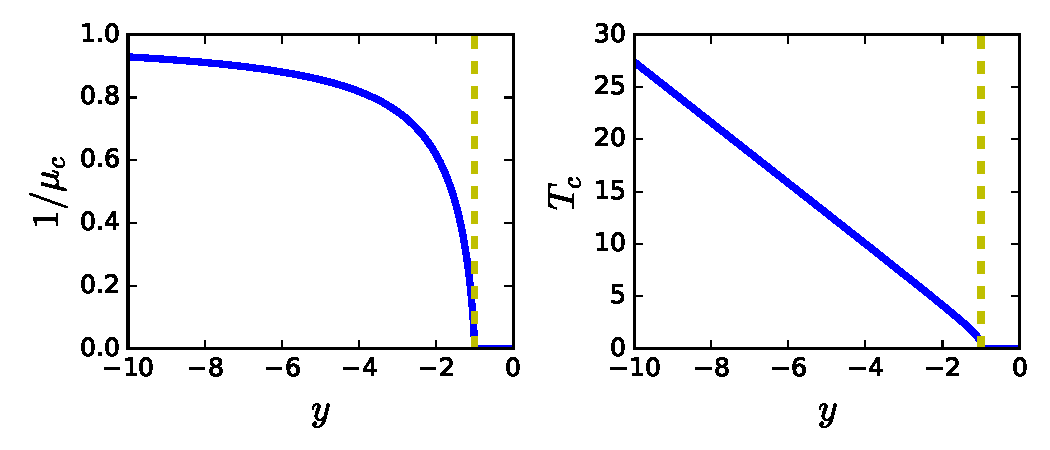
\includegraphics[width=0.9\columnwidth]{Chapter-3/HN35ysTransVsY.pdf}
\protect\caption{Transition temperatures at different $y$'s. This is also a phase diagram. The phase above the curves is the paramagnetic phase while the phase below the curve is the ferromagnetic phase. }
\label{fig:afm-hn35transys} 
\end{figure}

As shown in Fig. \ref{fig:afm-HN35KJ_ys}, $\kappa^*$ changes with temperature $\mu$. Similarly to FM Ising model \cite{Boettcher2011HNNP}, the values of $\mu$ satisfying $\kappa(\mu)=0$ are the phase transition temperatures. After transformation of Eq. \ref{eq:afm-fyps_k}, the equation $\kappa(\mu)=0$ can be rewritten as 
\begin{equation}
\mu^{1+y} + \mu^y -1 =0
\end{equation}
where there is a real root for $y\le-1.0$ in the antiferromagnetic range of $\mu>1$.  The transition temperature ($\mu_C$ or $T_C$) as a function of $y$ is shown in Fig.  \ref{fig:afm-hn35transys}.


\subsubsection{ HNNP, HN6, and their interpolations }

In the AFM scenario, for HNNP ($y = 0$), there are only 2 possible fixed points 
\begin{equation}
\kappa^* = 0, \ \lambda^* = \mu^2 
\end{equation} 
\begin{equation}
\kappa^* = \lambda^* = 1 
\end{equation} 
 The stability of HNNP is not uniform across different temperatures. The fixed point of $\kappa$ and $\lambda$ is 1 for $\mu \le 3$ ($T\ge1.820478\cdots$) and oscillating fixed points for $\mu > 3$ ($T<1.820478\cdots$). This result is obtained from both numerical iterations of $\kappa^*(\kappa, \lambda)$ and fixed point stability analysis from the Jacobian.
The simple numerical iterations of Eq. \ref{eq:afm-hpsol1} is shown in Fig. \ref{fig:afm-hnnpkappa}, and the absolute eigenvalue of Jacobian matrix is shown in Fig. \ref{fig:afm-hnnp_eigs}.
\begin{figure}
\centering 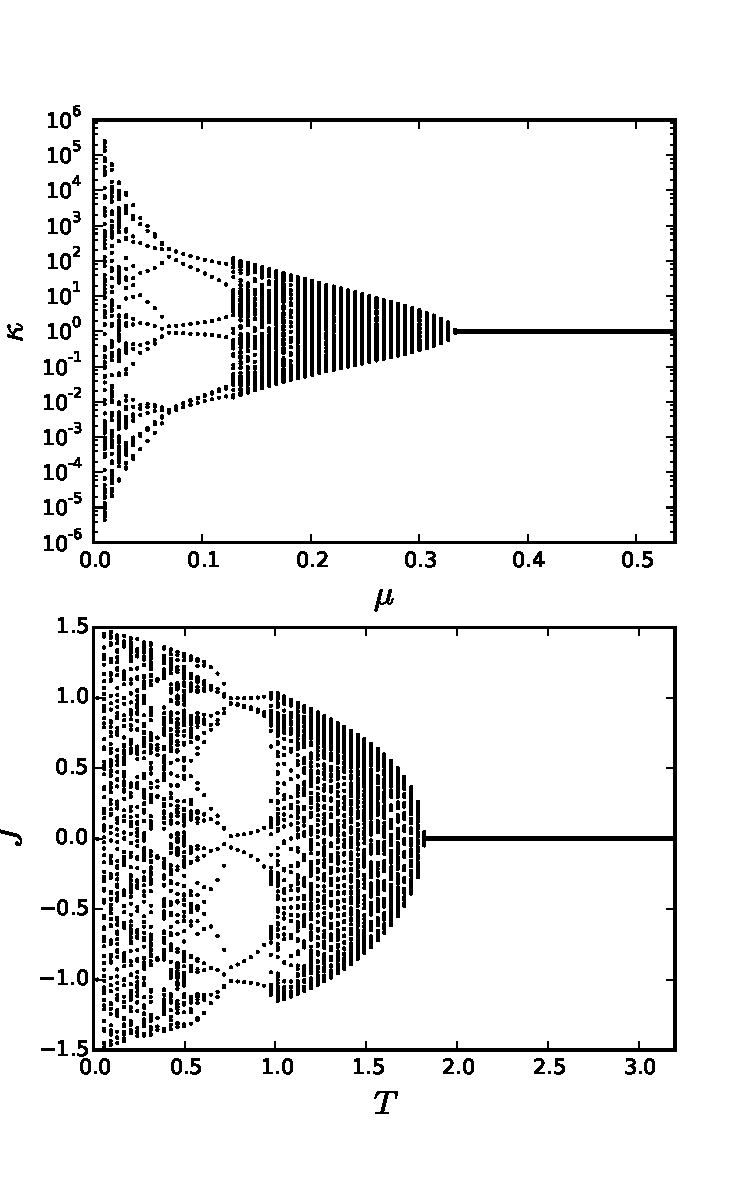
\includegraphics[width=0.6\columnwidth]{Chapter-3/HNNP_RG_Kvsmu_JvsT.pdf}
\protect\caption{ $\kappa$ and $J$ of HNNP RG recrusive numerical results. When $1/\mu < 1/3$ or $T < 2/\log(3)$, there is no stable fixed point. }
\label{fig:afm-hnnpkappa} 
\end{figure}


Similarly to the approach in HN3 and HN5, the Jacobian matrix of the recursive equations is
\begin{equation}
J_{11} = \frac{\partial \kappa'(\kappa, \lambda)}{\partial \kappa}=\frac{\lambda  (\mu +1)^2}{(\kappa  \mu +1)^2}-\frac{2 \kappa  \lambda  \mu  (\mu +1)^2}{(\kappa  \mu +1)^3}
\end{equation}
\begin{equation}
J_{12} = \frac{\partial \kappa'(\kappa, \lambda)}{\partial \lambda}=\frac{\kappa  (\mu +1)^2}{(\kappa  \mu +1)^2}
\end{equation}
\begin{equation}
J_{21} = \frac{\partial \lambda'(\kappa)}{\partial \kappa}=\frac{2 (\kappa +\mu ) }{(\kappa  \mu +1)^2}-\frac{2 (\kappa +\mu )^2 \mu }{(\kappa  \mu +1)^3}
\end{equation}
\begin{equation}
J_{22} = \frac{\partial \lambda'(\kappa)}{\partial \lambda}=0
\end{equation}
The 2 eigenvalues are 
\begin{eqnarray}
J_{\rm evig} = -\frac{(\mu +1)}{2 (\kappa  \mu +1)^3} \Big[\lambda  \mu  (\kappa +\kappa \mu -1)-\lambda \pm \nonumber \\ 
\sqrt{\lambda ^2 (\mu +1)^2 (\kappa  \mu -1)^2-8 \kappa  \left(\mu ^2-1\right) (\kappa +\mu ) (\kappa  \mu +1)} \Big] \nonumber \\
\label{eq:afm-hpeig}
\end{eqnarray}

\begin{figure}
\centering 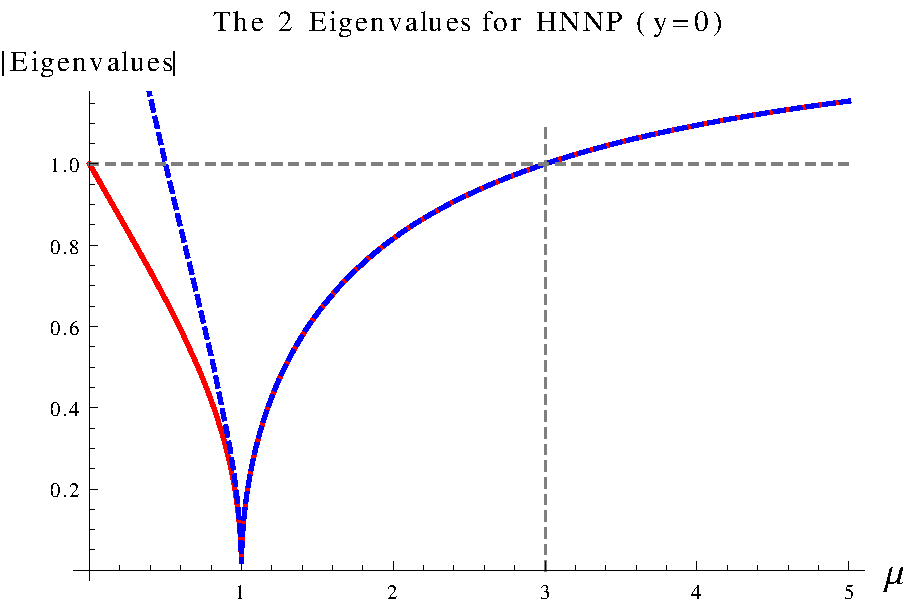
\includegraphics[width=0.6\columnwidth]{Chapter-3/HNNP_eigenvalues.pdf}
\protect\caption{The absolute values (1st norm) of the 2 complex eigenvalues for HNNP. For $0<\mu<1$, that is for the ferromagnetic case; while the antiferromagnetic region is $\mu>1$. You see the transition temperature is $\mu_g=3.0$ or $T_g=2/\log(3)=1.820478...$ because after that the $|{\rm eigenvalue}|>1$ . }
\label{fig:afm-hnnp_eigs} 
\end{figure}

\begin{figure}
\centering 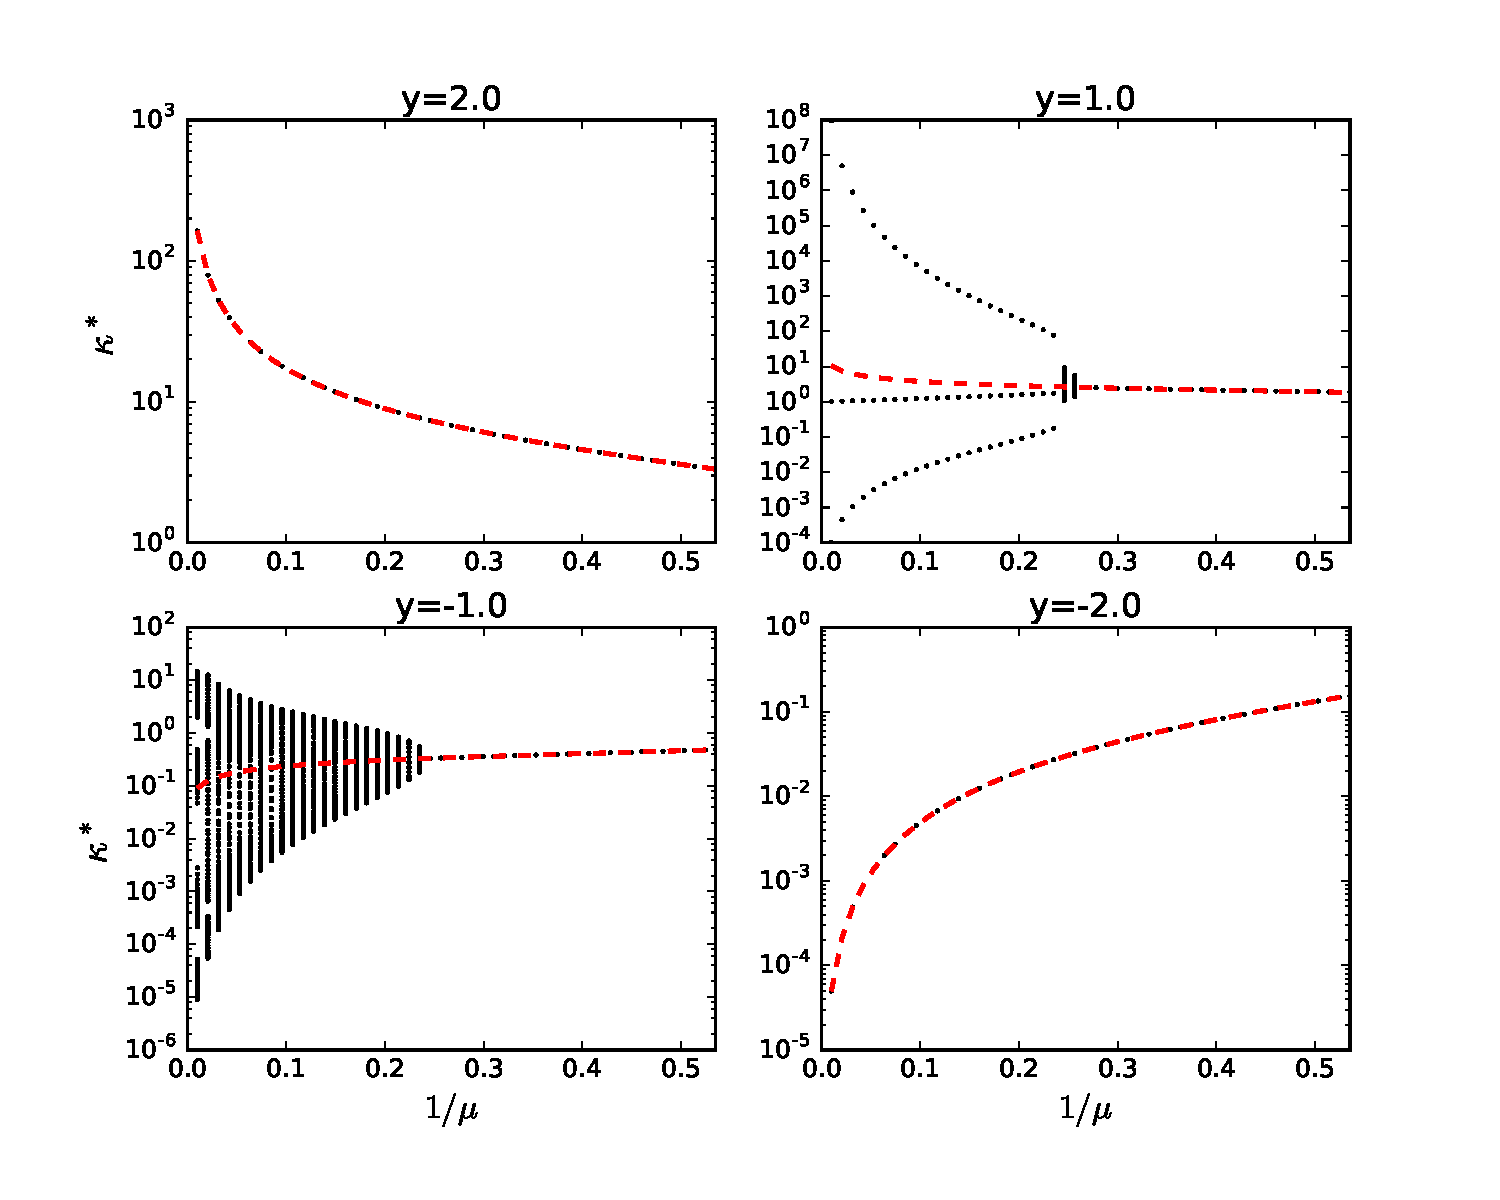
\includegraphics[width=1.0\columnwidth]{Chapter-3/HNP6_KvsMu_ys.pdf}
\protect\caption{Numerical iterations (dotted black) and analytical (red dashed) fixed points of $\kappa$. The numerical solutions are data points between RG steps $20,000$ and $20,100$. There is a chatoic transition for $-2.0<y<2.0$. }
\label{fig:afm-hp6Kys} 
\end{figure}

\begin{figure}
\centering 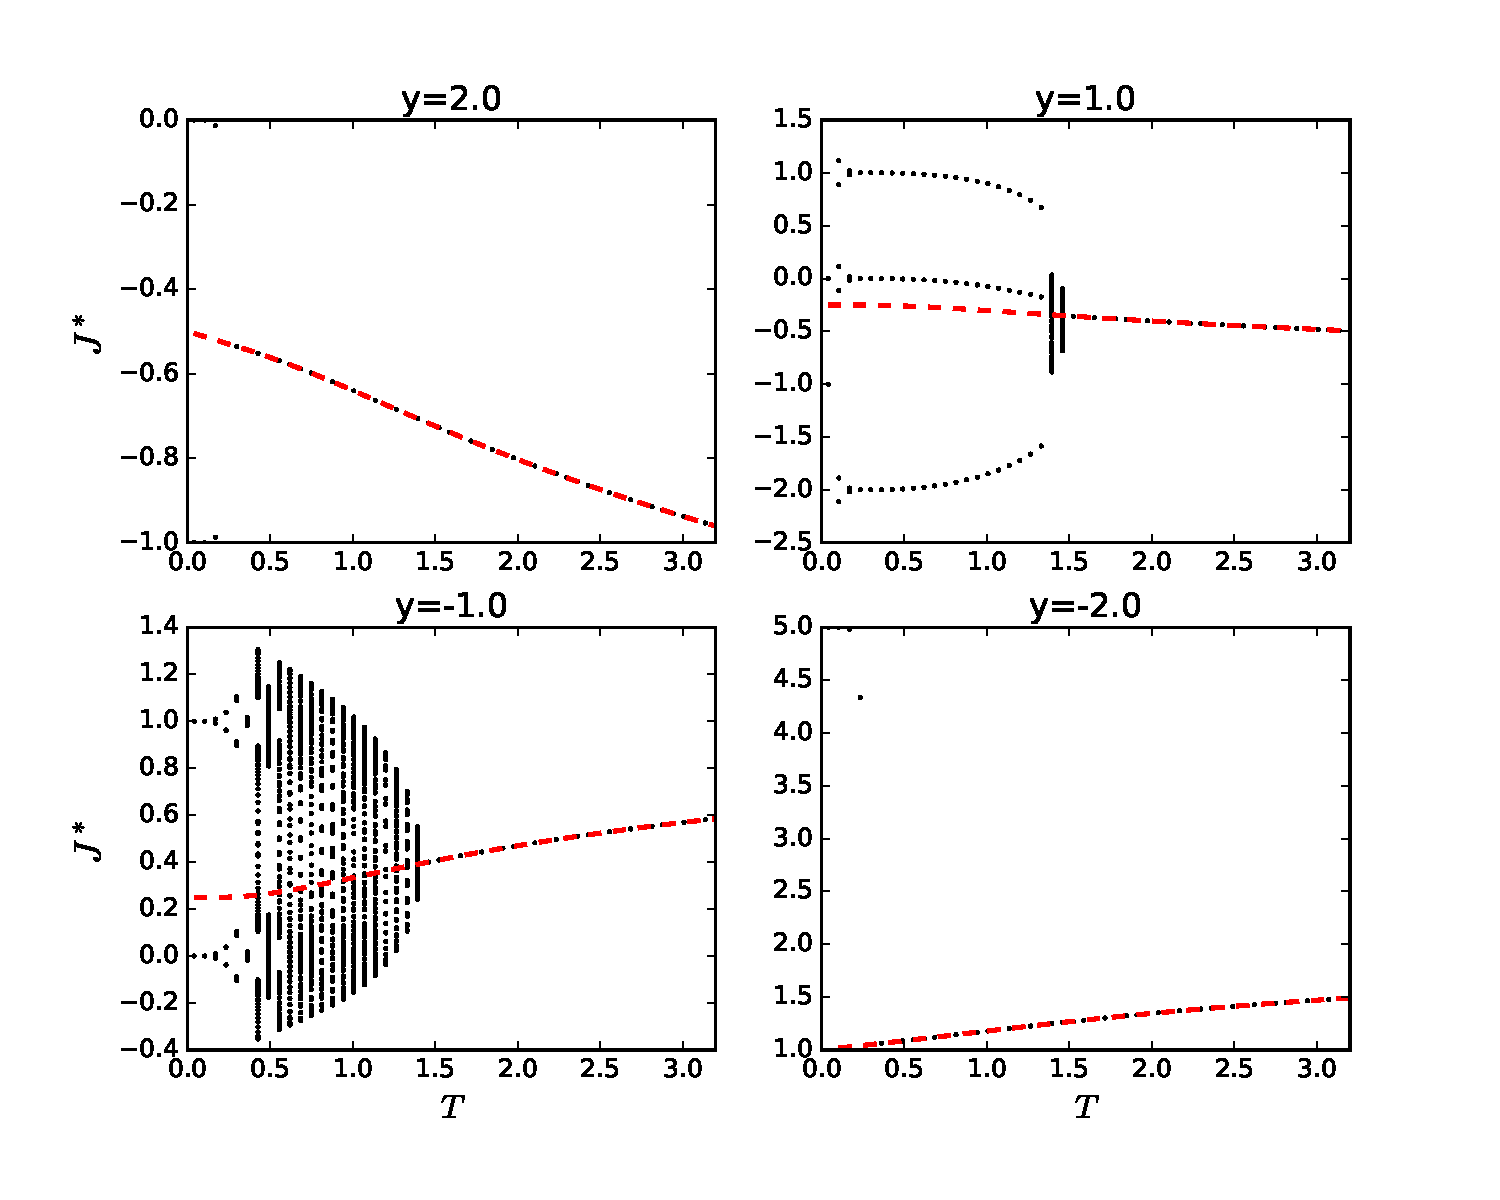
\includegraphics[width=1.0\columnwidth]{Chapter-3/HNP6_JvsT_ys.pdf}
\protect\caption{Numerical iterations (dotted black) and analytical (red dashed) fixed points of $J$. The numerical solutions are data points between RG steps $20,000$ and $20,100$. There is a chatoic transition for $-2.0<y<2.0$. At $y=\pm 2.0$, all the data points of numerical and analytical fixed points should exactly agree. The discrepancies at low temperatures is due to the finite numerical iterations. The discrepancies converge to 0 at infinite iterations which is to the thermodynamic limit.}
\label{fig:afm-hp6Jys} 
\end{figure}

We can plug in the 2 possible fixed points to these two eigenvalues, and the eigenvalues become
\begin{equation}
J_{\rm evig} = \frac{\pm \sqrt{-7 \mu ^2-2 \mu +9}-\mu +1}{2 \mu +2}
\label{eq:afm-hnnpJevig2}
\end{equation}
Because $\mu>1$ for AFM, the eigenvalues are complex numbers. In this case, the absolute values matter: if the absolute value is smaller than 1, there is a stable fixed points, otherwise there is not. The complex number means that the unstable fixed points are oscillating. More descriptions of the chaotic fixed points is included for generalized $y$'s later in this section. As shown in Fig. \ref{fig:afm-hnnp_eigs}, by solving the Eq. \ref{eq:afm-hpeig} $ ==1$, we can get the transition temperature is $\mu_g=3$ ($T_g=1.820478...$).


In this scenario, $y$ makes the fixed point much more complicated. One of the fixed point is
\begin{equation}
\kappa^* = 0, \ \ \lambda^* = \mu^{2+2y} 
\end{equation} 
Another positive fixed point for $\mu>1$ is 

\begin{equation}
\begin{array}{l}
\kappa^*=\frac{-2 \mu +\mu^{y/2}(\mu + 1) \left( \mu^{y/2}+\sqrt{4 (\mu -1) \mu +\mu ^y}\right) } {2 \mu ^2}  \\ \\
\lambda^* = \frac{1}{2} \mu ^{y-2} \left(2 (\mu -1) \mu +\mu ^y+\mu ^{y/2}\sqrt{4 (\mu -1) \mu +\mu ^y} \right) \\
\end{array}
\end{equation} 

Most interestingly, the fixed points are also chaotic for $-2<y<2$ (as shown in Fig. \ref{fig:afm-hp6Kys} and \ref{fig:afm-hp6Jys}).  When $y>2$, other links is relatively weak, and the model becomes fairly simple and has no phase transition. When $y<-2$, the whole system became similar to ferromagnetic model and have FM-like phase transitions (as shown in Fig. \ref{fig:afm-hp6KJnegy}). As shown in Fig. \ref{fig:afm-hp6KJnegy}, we can find the FM-like transition temperatures by solving $\kappa^*==0$  for $y<-2.0$, which is equivalently the solutions of 
\begin{equation}
1 - \mu^{1 + y} - \mu^{2 + y} = 0 
\end{equation}


\begin{figure}
\centering 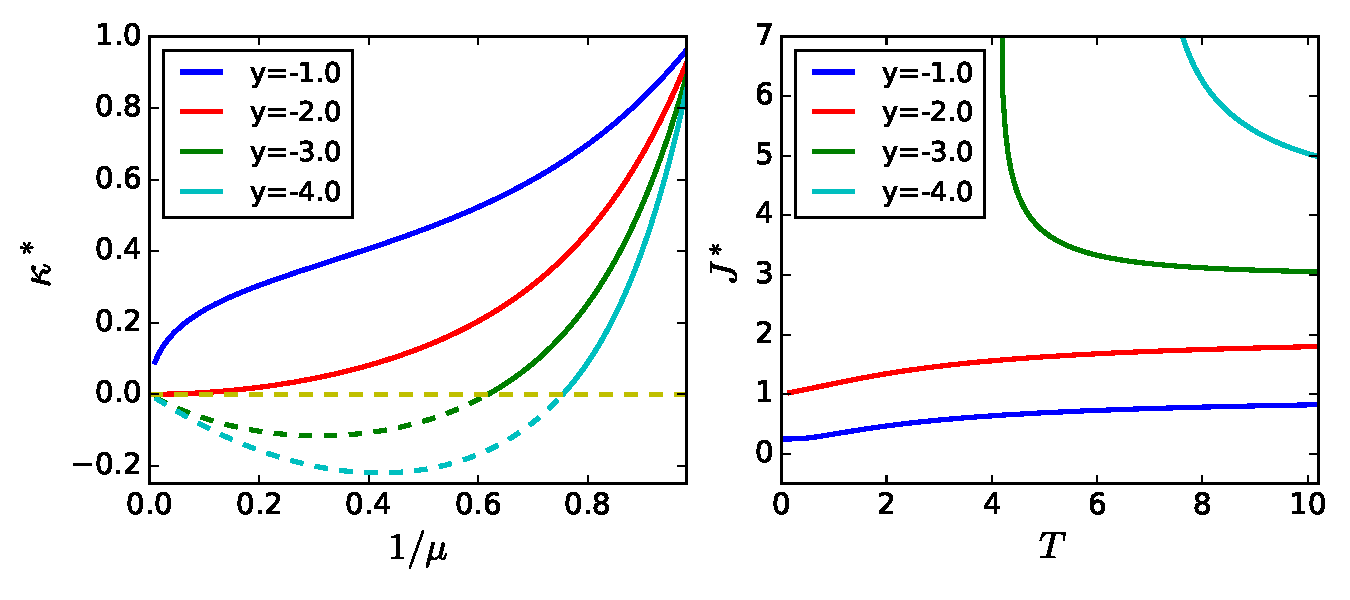
\includegraphics[width=1.0\columnwidth]{Chapter-3/HP_KJvsTys_FMTrans.pdf}
\protect\caption{Analytical (red dashed) fixed points of $\kappa$ and $J$ with different $y$'s. The solid curves are real and positive fixed points; while the dashed curves are negative ones. The 0 fixed points is the FM-like transition points.}
\label{fig:afm-hp6KJnegy} 
\end{figure}

\begin{figure}
\centering 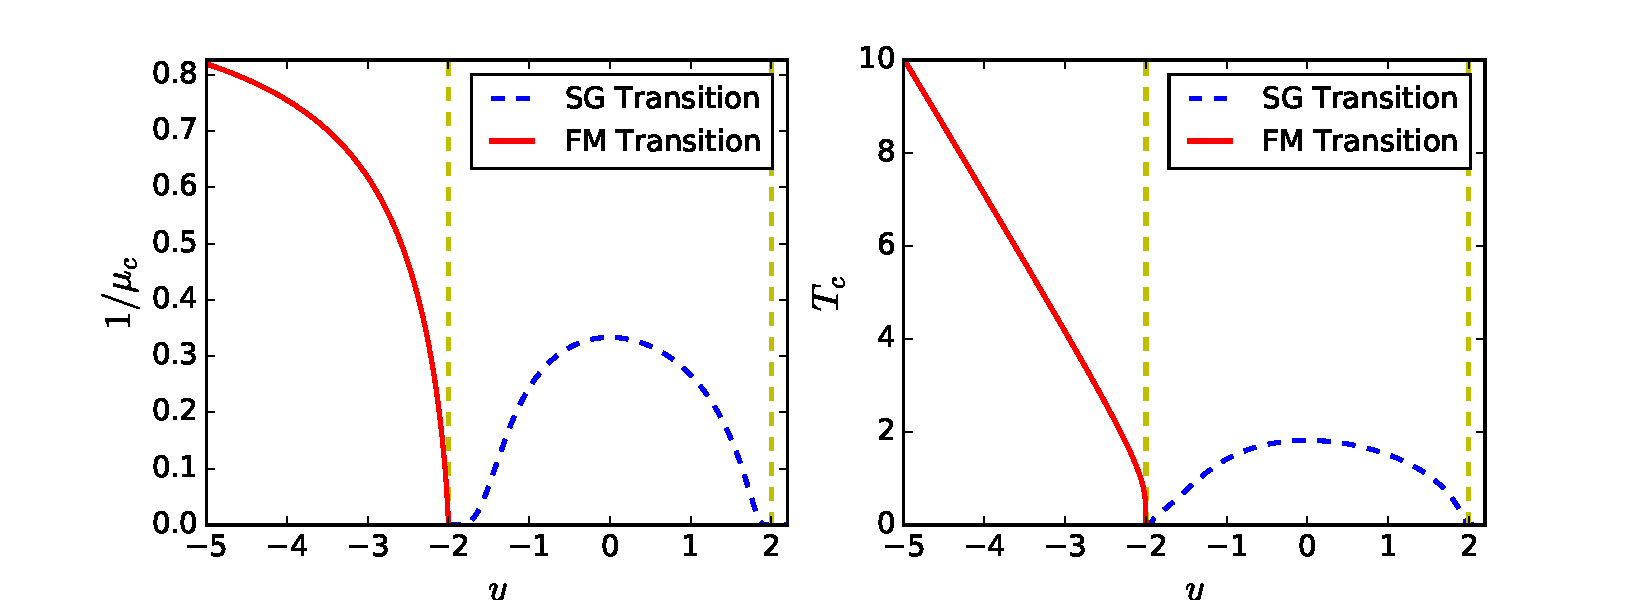
\includegraphics[width=1.0\columnwidth]{Chapter-3/HN6_TransTvsY1.pdf}
\protect\caption{Numerical Solution of chaotic transition temperatures and phase transition temperatures at different $y$'s for HNNP and HN6 interpolations. }
\label{fig:afm-hp6Tys} 
\end{figure}

The chaotic transition temperatures $T_g$ can be determined from the eigenvalues of the Jacobian matrix.
The Jocobian matrix is
\begin{equation}
J_{11} = \frac{\partial \kappa'(\kappa, \lambda)}{\partial \kappa}=\frac{\lambda  (\mu +1)^2}{(\kappa  \mu +1)^2}-\frac{2 \kappa  \lambda  \mu  (\mu +1)^2}{(\kappa  \mu +1)^3}
\end{equation}
\begin{equation}
J_{12} = \frac{\partial \kappa'(\kappa, \lambda)}{\partial \lambda}=\frac{\kappa  (\mu +1)^2}{(\kappa  \mu +1)^2}
\end{equation}
\begin{equation}
J_{21} = \frac{\partial \lambda'(\kappa)}{\partial \kappa}=\frac{2 (\kappa +\mu ) \mu ^{2 y}}{(\kappa  \mu +1)^2}-\frac{2 (\kappa +\mu )^2 \mu ^{2 y+1}}{(\kappa  \mu +1)^3}
\end{equation}
\begin{equation}
J_{22} = \frac{\partial \lambda'(\kappa)}{\partial \lambda}=0
\end{equation}

The transition temperature can be solved by setting an equation of $\rm |eigenvalue|==1$. The explicit equations of the eigenvalues are not shown due to length and complexity. Because the 2 eigenvalues are conjugate complex numbers, $\rm |eigenvalue|$ is the 1st norm. For complex eigenvalues, if the 1st norm is smaller than 1, the recursive equations can reach a stable fixed point; otherwise, it would not. Also, complex eigenvalues usually mean oscillating flow of the parameters, which is what we see in the numerical iterations in Fig. \ref{fig:afm-hp6Kys}.
The equation of $\rm |eigenvalue|==0$ is not solvable analytically but can be numerically solved to find the chaotic transition temperatures. The transition temperatures at different $y$'s are shown in Fig. \ref{fig:afm-hp6Tys}




\subsection{Equilibrium Properties}
\label{sec:afm-eqa}
Equilibrium properties are vital to learn critical phenomena and almost impossible to study experimentally for glassy systems due to the extremely long relaxation. To learn the equilibrium properties of AFM in Hanoi networks, there are 2 methods: Wang-Landau sampling and/or RG. 

\begin{figure}
\centering 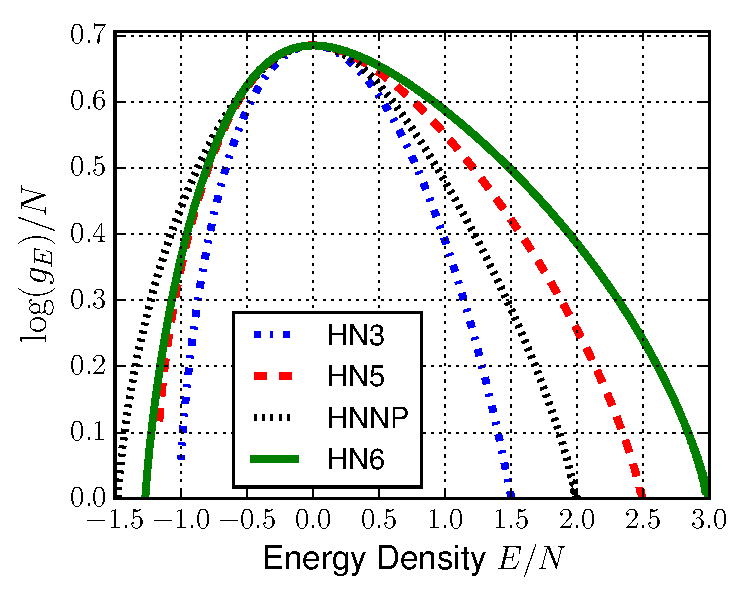
\includegraphics[width=0.6\columnwidth]{Chapter-3/HN35P6DOS_h3.pdf}
\protect\caption{Density of states from Wang-Landau sampling for system size $N=512$. Both the planar networks have highly degenerated ground states; while the nonplanar ones have unique ground states. This is also confirmed by the entropy from RG. }
\label{fig:afm-doswl} 
\end{figure}

Wang-Landau sampling can estimate the density of states $g_E$, which yields the partition function as 
\begin{equation}
Z(\beta)=\sum_{i=1}^{N_{E}}g_{E_i}e^{-\beta E_i}
\end{equation}
where $\beta$ is $1/T$, and $N_E$ is the total number of energy states. The density of states for different HNs in AFM are shown in Fig. \ref{fig:afm-doswl}. We can see there is clearly a difference between planar (HN3, HN5) and nonplanar networks (HNNP, HN6). The planar networks have highly degenerate ground states, which may indicate more glassy dynamics at low temperature. The nonplanar networks have unique ground state, which may indicate an equilibrium phase transition. The ground states degenency can be further proved by the entropy density $s$ from RG as shown in Fig. \ref{fig:afm-entropy}. However, the Wang-Landau sampling can only converge for system sizes $<1024$. Due the small system sizes in Wang-Landau sampling's results, no evidence is obtained to prove the speculations of phase transitions.
Therefore, RG is needed to reach any meaningful conclusion for systems in the thermodynamic limit.

\begin{figure}[h]
\centering 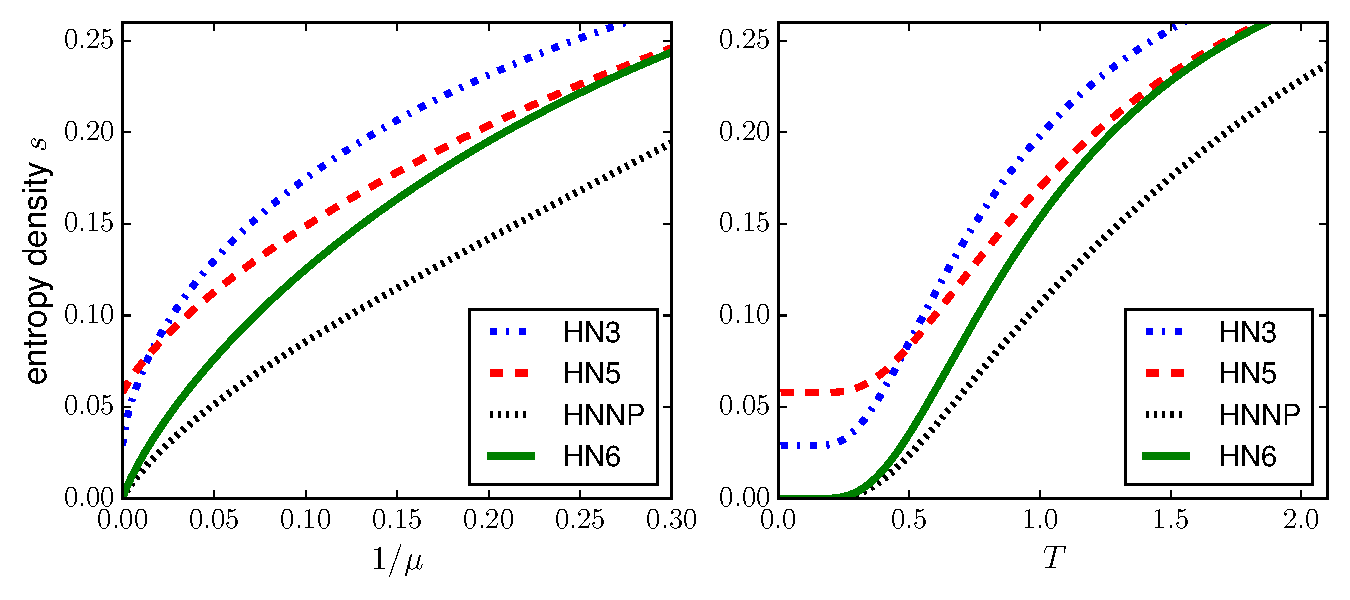
\includegraphics[width=0.88\columnwidth]{Chapter-3/HNs_entropy_density.pdf}
\protect\caption{Entropy Densities for all HNs of system sizes $N=2^{16}, 2^{32}, 2^{64}$. Each Hanoi network has 3 curves of different system sizes, and these curves all cllapses on each other, which shows these curves can represent the behavior in the thermodynamic limit.  }
\label{fig:afm-entropy} 
\end{figure}

\begin{figure}[h]
\centering 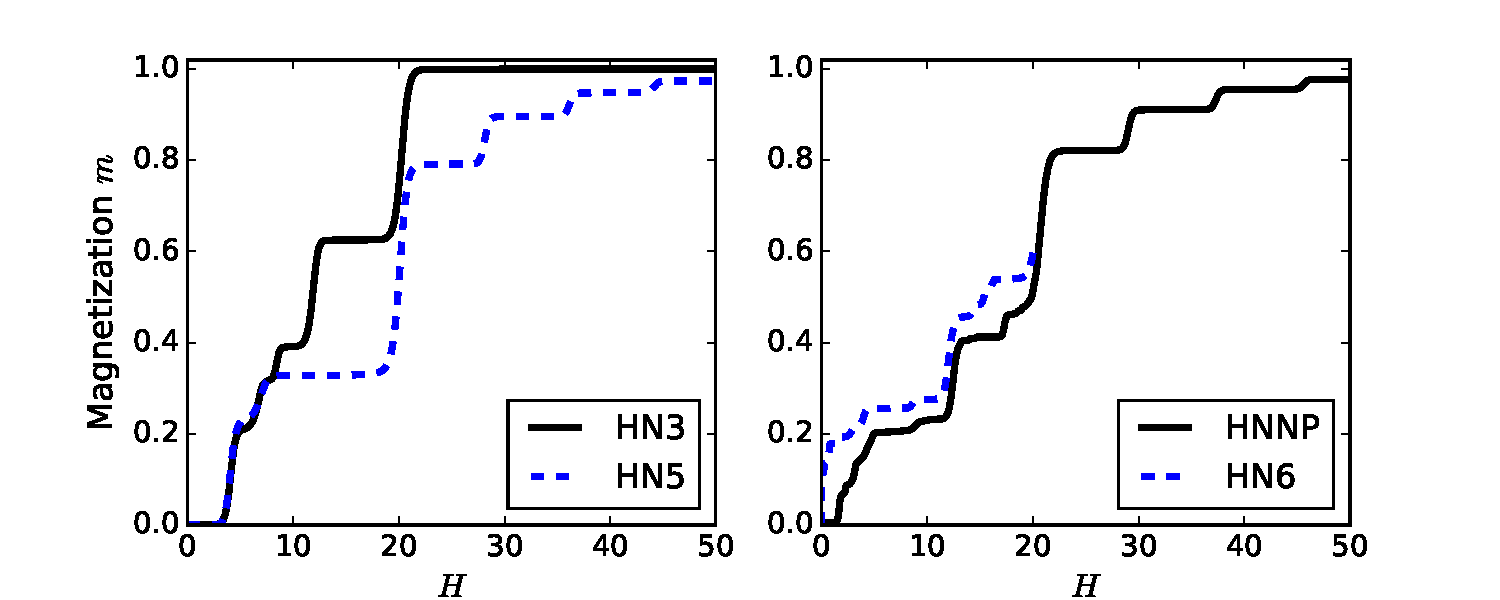
\includegraphics[width=0.9\columnwidth]{Chapter-3/HNs_MagvsH_m_vs_H.pdf}
\protect\caption{Magnetization patterns with increasing external magnetic fields at low temperature $T=0.1$ for system size $N=2^{128}$ using RG.}
\label{fig:afm-magplt}
\end{figure}

Using RG, we explored most common physical properties, such as internal energy per spin $\langle e\rangle$, magnetization per spin $\langle e\rangle$, free energy $\langle e\rangle$ with different boundary conditions, specific heat, susceptibility. Our interesting findings are described as follows.

The results of the internal energy have been included in Sec. \ref{sec:afm-dyn} and show the glassy dynamics ( Fig. \ref{fig:afm-hnsjam} ) sand the power-law relaxation (Fig. \ref{fig:afm-hnsscaling}). 

Another interesting finding is the magnetization behavior as to the increasing external
 magnetic field. The plateau patterns similar to others' findings \cite{ohanyan2003mag} have
 been found as shown in Fig. \ref{fig:afm-magplt}. These plateaus may be because of the
 hierarchically distributed local spin pattern. Specifically, the overall average magnetization per
 spin is zero, but the local spin-generated fields are non-zero and may be correlated with the
 Hanoi networks' hierarchy. These local non-zero fields may have a nonuniform discrete
 distribution, which leads to the plateaus with different lengths. Often, these magnetization
 plateaus are believed to be from quantum effects 
\cite{kageyama1999pleatu, kageyama2000direct}. This result provides another example of
 classical system where the plateaus are mainly caused by the structure of the networks. 
Further conclusion needs detailed information of the low-temperature (even ground states)
 spin configuration, which is not directly retrievable from RG.

\begin{figure}
\centering 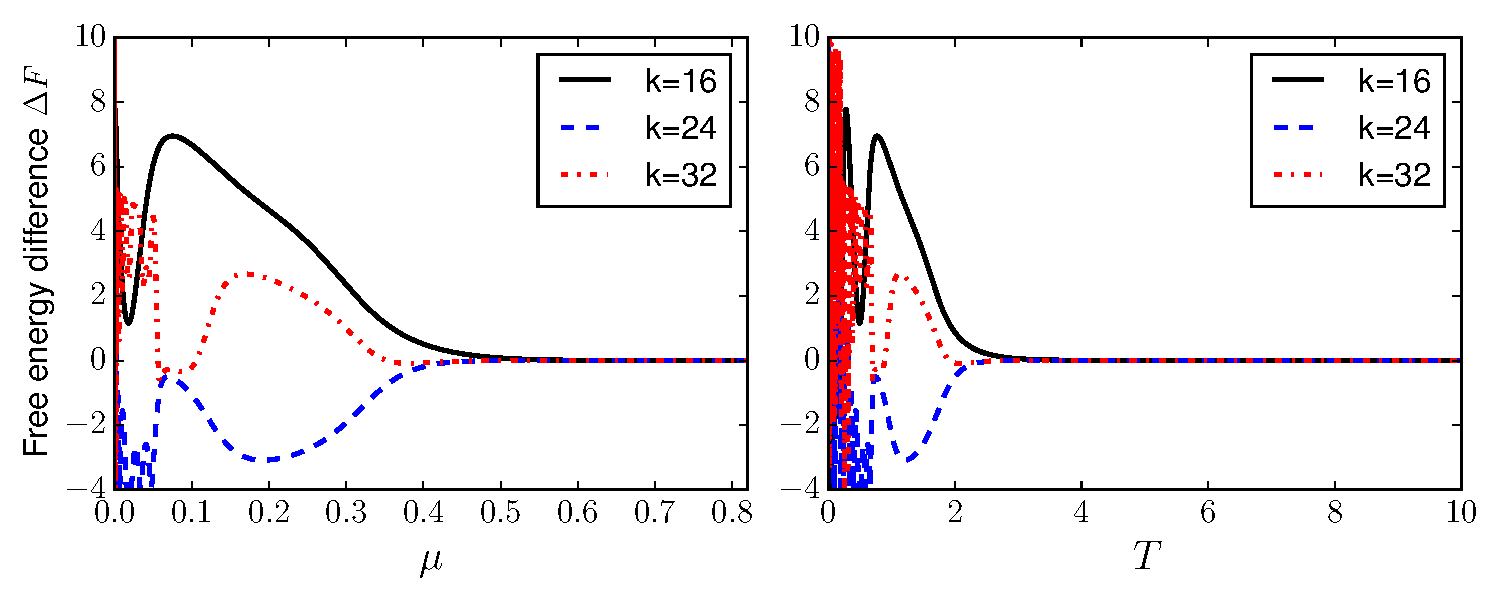
\includegraphics[width=1\columnwidth]{Chapter-3/freeE_lowT2highT.pdf}
\protect\caption{The free energy difference between the 2 boundaries conditions at different temperatures. The system size is $N=2^k$, which are $2^{16}$, $2^{24}$, $2^{32}$ in the figure above. Obviously, at higher temperatures, there is no difference; at low temperatures, there is more and more difference variations for bigger and bigger system sizes. A plot for low $T$ is shown next (Fig. \ref{fig:afm-freeEdiff}) which shows the chaos at low $T$.  }
\label{fig:afm-freeEdiff_allT} 
\end{figure}

One of the main goals of RG is to explore the chaotic behaviors found in the fixed point analysis.
 In AFM, the free energy with different boundary conditions has been used to study the chaos in physical systems. The reference parameter is the free energy difference $\Delta F$ (Eq. \ref{eq:afm-freediff}) between different boundary conditions. The difference at a wide range of temperatures are shown in Fig. \ref{fig:afm-freeEdiff_allT} which shows the $\Delta F$ is 0 at high $T$ but non-zero and chaotic at low $T$. The curves may have very different patterns for difference system size, and Fig. \ref{fig:afm-freeEdiff}  is an example. 

\begin{figure}
\centering 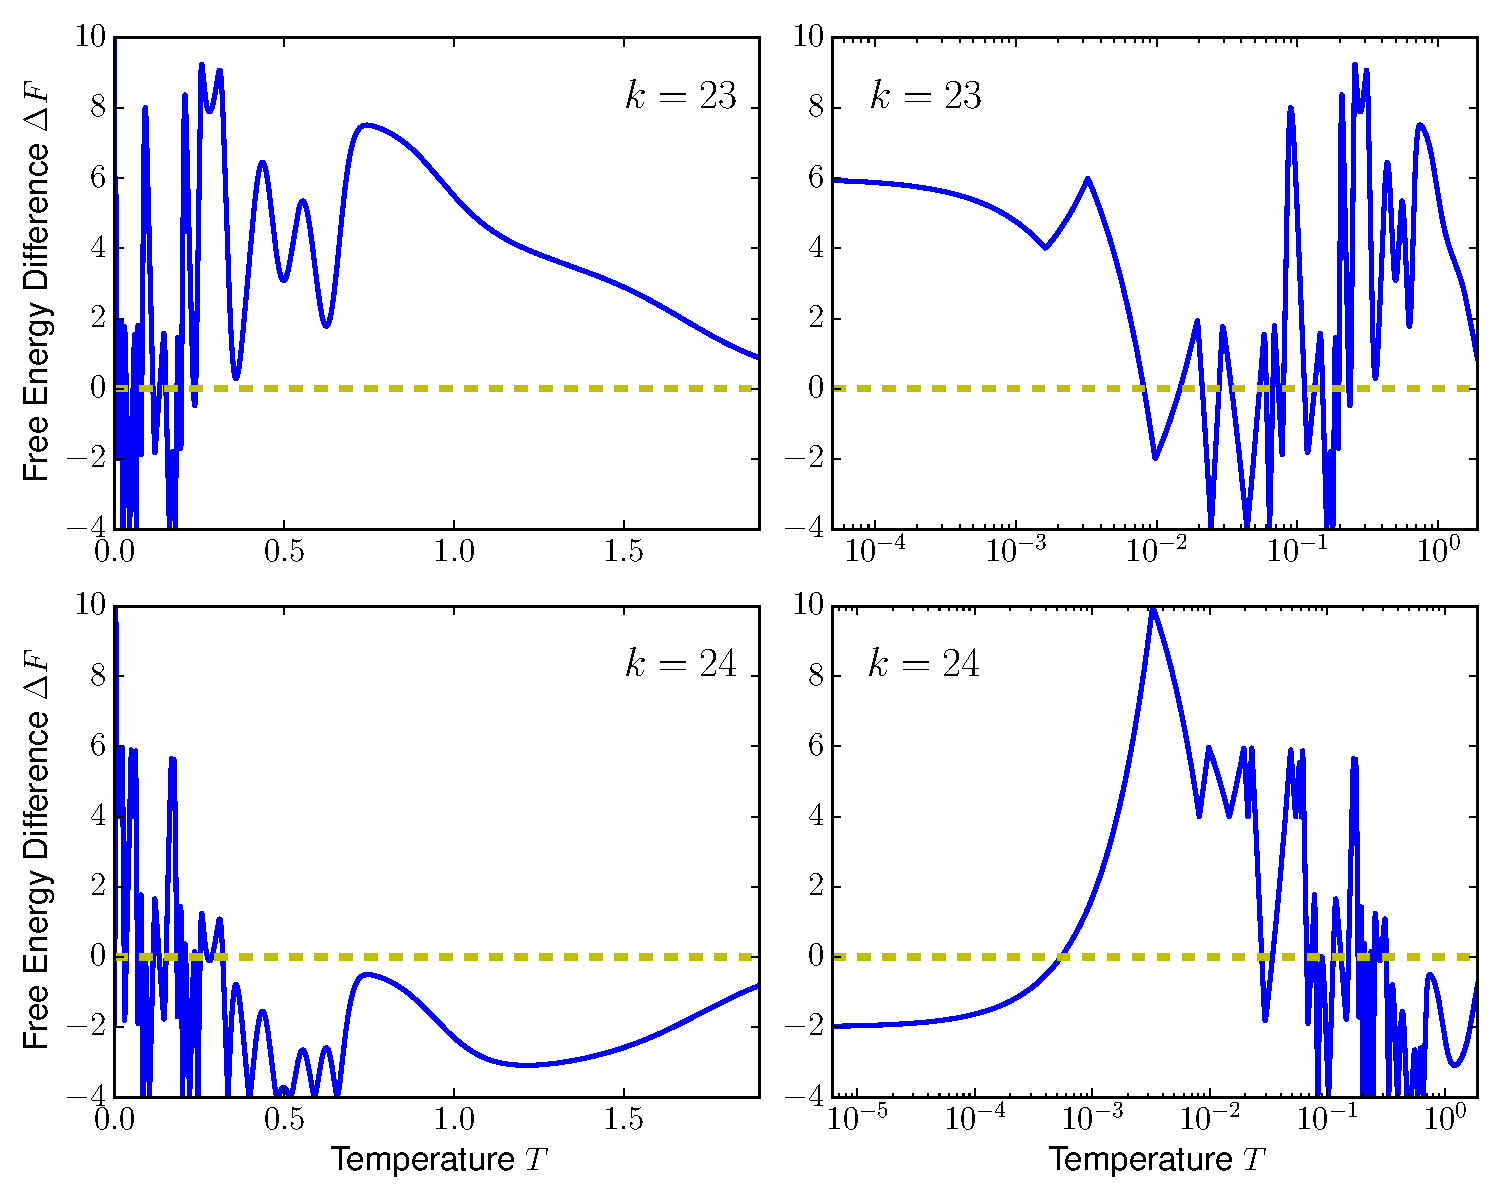
\includegraphics[width=0.8\columnwidth]{Chapter-3/freeEdifference_k23_24.pdf}
\protect\caption{The free energy difference between the 2 boundaries conditions at low temperatures $T<2.0$. The yellow dashed line is to show where the crossings of $f_1$ and $f_2$ are. ($f_1$: parallel boundary condition; $f_2$: anti-parallel boundary condition.) }
\label{fig:afm-freeEdiff} 
\end{figure}

\begin{figure}
\centering 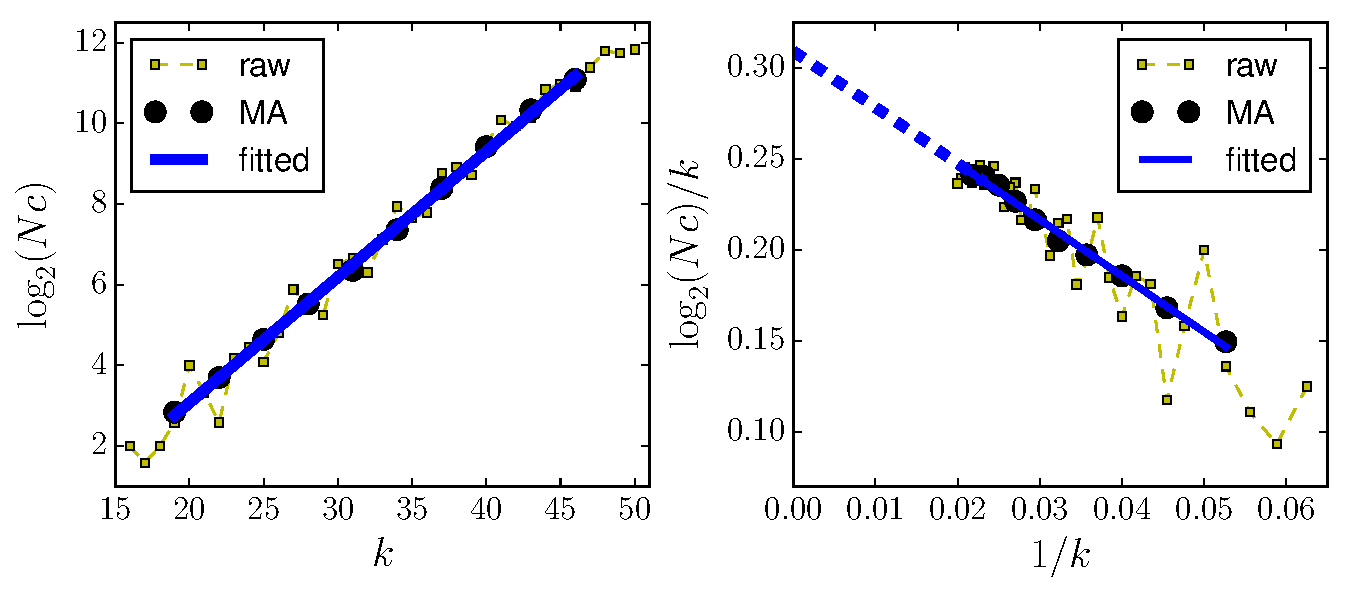
\includegraphics[width=0.8\columnwidth]{Chapter-3/chaotic_exponents_freeE_binning.pdf}
\protect\caption{Number of free energies crossings fitted to $k$ (=$\log_2 N$) in the temperature range $T \in [10^{-3}, T_g]$ for HNNP. The yellow squares are the raw $N_c$'s which have fluctuations due to finite size scaling and numerical precision. To get a more reliable fitting, the moveing average (black circles) with window size of 6 and overlap of 3 are used for fitting. Two methods of fitting are used: Eq. \ref{eq:afm-fit1} (left figure) and Eq. \ref{eq:afm-fit2} (right figure). The exponents are $0.312\pm 0.003$ and $0.309 \pm 0.003$, respectively. Both of the $R^2$ is bigger than $0.99$.}
\label{fig:afm-freeEfit} 
\end{figure}

The crossing point is where $\Delta F = 0$ and $\Delta F$ changes sign. In other words, $f_1$  (parallel boundary condition) and $f_2$ (anti-parallel) switch their order. In a spin glass with chaotic dynamics, the number of crossings $N_c$ is expected to increase polynomially with system size 
\begin{equation}
N_c = A N^\alpha
\end{equation}
where $A$ is a constant, $N$ is the system size, and $\alpha$ is the exponent. The exponent $\alpha$ is called chaotic exponent. There is two way to obtain chaotic exponent $\alpha$. The first way is 
\begin{equation}
\log_2 N_c = \log_2 A + \alpha \log_2 N
\label{eq:afm-fit1}
\end{equation}
, and the second way is 
\begin{equation}
\frac{\log_2 N_c }{\log_2 N } =\frac {\log_2 A }{\log_2{N}} + \alpha 
\label{eq:afm-fit2}
\end{equation}
where $\log_2 N = k$. The two ways can show us the trend from different perspectives as shown in Fig. \ref{fig:afm-freeEfit}. 
These two exponents are $0.312\pm 0.003$ and $0.309 \pm 0.003$, respectively. Both strongly show there is a power-law increase with system size. 

As you may notice from the free energy curves in Fig. \ref{fig:afm-freeEdiff}, $N_c$ may dependent on the temperature and step size. First, we tested different 2 more temperatures ranges $T \in [0.1, 0.2]$ and $T \in [0.2, 0.3]$ which show similar pattern. Second, different step sizes are tested to make sure the $N_c$ does not change with a smaller step size. 


\section{Summary and Conclusion}

